\documentclass[11pt]{article}

\usepackage[a4paper,margin=1.2in]{geometry}
\usepackage{amsmath,amssymb,amsthm,mathtools}
\usepackage{hyperref}
\usepackage{booktabs}
\usepackage{enumitem}
\usepackage{tikz}
\usetikzlibrary{decorations.pathreplacing,calc,arrows.meta,patterns}
\usepackage[normalem]{ulem}

\hypersetup{colorlinks=true, linkcolor=blue!50!black, citecolor=blue!50!black}

% Independent counters, so that Theorem/Lemma/Proposition/Corollary numbers in this
% companion coincide with the corresponding numbers in the paper.
\newtheorem{theorem}{Theorem}
\newtheorem{proposition}{Proposition}
\newtheorem{lemma}{Lemma}
\newtheorem{corollary}{Corollary}
\theoremstyle{definition}
\newtheorem{definition}{Definition}
\theoremstyle{remark}
\newtheorem{remark}{Remark}

\newcommand{\E}{\mathbb{E}}
\newcommand{\Var}{\mathrm{Var}}
\newcommand{\Prob}{\mathbb{P}}
\newcommand{\R}{\mathbb{R}}
\newcommand{\dt}{\Delta t}
\newcommand{\1}{\mathbf{1}}
\newcommand{\bound}{\mathrm{bound}}
\DeclareMathOperator{\sgn}{sign}

\title{Study Companion: \\
The Mathematics of\\
\emph{Optimal Block Time for AMM Liquidity Providers\\
under Jump-Diffusion Prices}}
\author{Nils Bundi}
\date{}

\begin{document}
\maketitle
\tableofcontents
\vspace{1em}

\noindent\textit{This document is a step-by-step companion to the main paper. Where the paper is terse, this document is verbose: it spells out every line of algebra, states every assumption and says what it costs, and connects each derivation to the standard result it applies. Read it side-by-side with the paper.}

\medskip
\noindent\textbf{How to use this document.} The intended reader is a graduate student who wants to check the paper line by line. Three conventions help with that.
\begin{itemize}[leftmargin=2em]
\item Whenever an off-the-shelf theorem is used, it is cited to a specific numbered result---overwhelmingly to Cont and Tankov~\cite{cont2003financial} for the It\^o--L\'evy machinery, and to Milionis, Moallemi and Roughgarden~\cite{milionis2022automated,milionis2023automated} for the LVR framework this paper extends. Where a result is taken from another paper, that paper is named at the point of use.
\item Every assumption gets its own paragraph headed \textbf{Assumption}, stating what is assumed, why, and what is lost. Assumptions that are genuine restrictions are labelled as such and are \emph{not} presented as normalizations.
\item Section~\ref{sec:experiments} walks through each numerical experiment in \texttt{code.py}: what it computes, what it is a check on, and what it returns. Several results in the paper are asserted on the strength of these experiments rather than proved, and this document says which.
\end{itemize}

\medskip
\noindent\textbf{Notation.} The paper's notation is used throughout. Two symbols do a lot of work and are worth fixing now: $\kappa := \gamma/(\sigma\sqrt{\dt})$ is the fee measured in units of the per-block diffusive move, and $\eta := \sqrt2\,\kappa$ is the same quantity in the units in which the stationary law of Section~\ref{sec:stationary} is naturally written. A full table is at the end.

\bigskip
\hrule
\bigskip

\section{The setup}\label{sec:setup}

The setup has four pieces: the price process, the constant-product market maker, the arbitrageur, and the LVR definition. Each piece is a deliberate modeling choice. This section walks through every choice with its motivation.

\subsection{The price process}

The reference price $S_t$ is the price on a centralized exchange or oracle. It is the price the AMM is being arbitraged \emph{against}. We model it as a \emph{Merton jump-diffusion}:
\begin{equation}\label{eq:sde}
\frac{dS_t}{S_{t-}} \;=\; \mu\,dt + \sigma\,dW_t + (e^{J_t} - 1)\,dN_t.
\end{equation}

Let us read each piece very carefully.

\paragraph{Why a ratio, not a difference?}
The left-hand side is the \emph{percentage return}, $dS_t / S_{t-}$, not the absolute change $dS_t$. Modeling percentage returns rather than absolute changes makes the process \emph{geometric}: if $S_t$ is the price of an asset, then doubling the scale of the price (e.g., a stock split) should not change the statistics of returns. Working with $dS_t / S_{t-}$ enforces this scale invariance and prevents $S_t$ from going negative.

\paragraph{Why $S_{t-}$ in the denominator?}
The minus subscript means ``the value of $S$ immediately before time $t$.'' Formally:
\[
S_{t-} \;:=\; \lim_{s \uparrow t} S_s.
\]
If $t$ is not a jump time, $S_t = S_{t-}$ (the process is continuous there). If $t$ is a jump time, $S_t \neq S_{t-}$. The jump has happened by $t$, but not by $t-$.

We need this distinction because the integrand against $dS_t$ in stochastic integrals must be \emph{predictable}. That is, it must be known just \emph{before} a jump, not at or after it. If we wrote $S_t$ in the denominator at a jump time, we would be ``cheating'' by using post-jump information to scale the pre-jump update.

\paragraph{The drift $\mu\,dt$.} A deterministic upward trend, like the expected return of a stock per unit time. For LVR analysis this term will turn out not to matter: LVR is a \emph{quadratic-variation} quantity that depends only on the second-order behavior of the price, not on the drift. We will keep $\mu$ in the model for generality but it will drop out of every result.

\paragraph{The Brownian increment $\sigma\,dW_t$.} Here $W_t$ is a standard Brownian motion (in particular, $dW_t \sim \mathcal{N}(0, dt)$ over a small interval $dt$, and increments over disjoint intervals are independent). The coefficient $\sigma$ is the \emph{instantaneous volatility} of returns: over a small interval $dt$, the conditional variance of $dS_t / S_{t-}$ contributed by the Brownian part is $\sigma^2\,dt$. Between jumps, $S_t$ behaves like a geometric Brownian motion (the Black–Scholes model).

\paragraph{The jump term $(e^{J_t} - 1)\,dN_t$.}
This is the new ingredient relative to Black–Scholes. Two objects appear:
\begin{itemize}[leftmargin=2em]
\item $N_t$ is a \emph{Poisson process} with intensity $\lambda > 0$. This means: the times $\tau_1 < \tau_2 < \cdots$ at which $N$ increases by $1$ are random, the inter-arrival times $\tau_{i+1} - \tau_i$ are i.i.d.\ exponential with mean $1/\lambda$, and the expected number of jumps in any interval of length $T$ is $\lambda T$.
\item $J_t$ is the \emph{log-jump size}. At each Poisson tick $\tau_i$, a random number $J_{\tau_i}$ is drawn (independently of everything that came before) from a fixed distribution: $J \sim \mathcal{N}(m, \delta^2)$. We call this the \emph{Merton} specialization. (Other choices: Kou (2002) uses an asymmetric double-exponential; we will see just below that the SDE structure is identical regardless of the choice of jump distribution.)
\end{itemize}

The product $(e^{J_t} - 1)\,dN_t$ is zero between jumps and equals $e^{J_{\tau_i}} - 1$ at the $i$-th jump. So at the jump time $\tau_i$, the relative price change is
\[
\frac{\Delta S_{\tau_i}}{S_{\tau_i-}} \;=\; e^{J_{\tau_i}} - 1, \qquad \text{i.e.,}\qquad S_{\tau_i} = S_{\tau_i-}\cdot e^{J_{\tau_i}}.
\]
A log-jump of size $J$ multiplies the price by $e^J$. If $J > 0$ the price jumps up. If $J < 0$ it jumps down. Because $S_{\tau_i-}$ is always positive and $e^J$ is always positive, the price stays positive. This is a desirable property.

\paragraph{The rigorous form of the jump term.}
The shorthand $(e^{J_t} - 1)\,dN_t$ in our SDE is informal but convenient. Written rigorously, the jump term is an integral against a \emph{Poisson random measure} $J$ on the product space $[0,\infty) \times \mathbb{R}$ (time axis, jump-size axis):
\[
\int_0^t \int_{\mathbb{R}} (e^y - 1)\,J(ds, dy) \;=\; \sum_{\tau_i \le t}(e^{J_{\tau_i}} - 1).
\]
The left-hand side is a continuous-looking integral. The right-hand side reveals what it actually computes: a sum over the (random) jump times $\tau_i$ with $(e^{J_{\tau_i}} - 1)$ as the summand. The two are the same object in different notations. The shorthand $(e^{J_t}-1)\,dN_t$ in equation~\eqref{eq:sde} packages this integral in differential form. At a jump time, $dN_t = 1$ and $J_t$ is the just-drawn mark. Elsewhere $dN_t = 0$ and the term contributes nothing.

\paragraph{What is a Poisson random measure, exactly?}
We used the term casually above. Here is the definition. An ordinary (deterministic) measure $\mu$ on a space $E$ assigns a non-negative number $\mu(A)$ to each measurable set $A \subseteq E$. For example, Lebesgue measure assigns each interval its length. A \emph{random measure} $M(\omega, \cdot)$ assigns a non-negative number $M(\omega, A)$ to each set $A$, but the number depends on the random outcome $\omega \in \Omega$. So $M(A)$ is itself a random variable for each fixed $A$.

The specific random measure relevant for our SDE lives on the product space $E = [0, \infty) \times \mathbb{R}$. It is constructed from the pair $(N_t, J_{\tau_i})$ as follows. At each Poisson tick $\tau_i$, a mark $J_{\tau_i} \in \mathbb{R}$ is independently drawn from the jump-size distribution $\nu$ (in our paper, $\nu = \mathcal{N}(m, \delta^2)$). The random measure $J$ then places one unit of mass at the point $(\tau_i, J_{\tau_i}) \in E$ for each $i$:
\[
J(\omega, A) \;:=\; \#\big\{i \;:\; (\tau_i, J_{\tau_i}) \in A\big\} \;=\; \sum_{i \ge 1} \mathbf{1}_A(\tau_i, J_{\tau_i}).
\]
So $J(A)$ counts how many ``time--jump-size'' pairs fall inside the set $A$. It is a \emph{Poisson} random measure because the counts $J(A_1), J(A_2), \ldots$ for disjoint sets are independent Poisson random variables. Its expected count is
\[
\E[J(A)] \;=\; \int_A \lambda\,ds\,\nu(dy),
\]
and the deterministic measure $\lambda\,ds\,\nu(dy)$ is called the \emph{intensity measure} (or \emph{compensator}) of $J$.

\paragraph{How integration against a random measure works.}
Integrals against $J$ are defined pathwise as sums over the points where $J$ has mass:
\[
\int_0^t \int_{\mathbb{R}} \phi(s, y)\,J(ds, dy) \;:=\; \sum_{\tau_i \le t} \phi(\tau_i, J_{\tau_i}).
\]
The integral notation looks continuous, but it really is a sum. The random measure $J$ only ``hits'' a discrete set of points. The expected value of such an integral, by the \emph{compensator formula}, is
\[
\E\!\left[\int_0^t\!\int \phi(s, y)\,J(ds, dy)\right] \;=\; \int_0^t \!\int \phi(s, y)\,\lambda\,ds\,\nu(dy).
\]
Conceptually: ``the expected sum over jumps equals the integral against the intensity.'' This is the standard identity used throughout the proof of Theorem~1 (the marked-Poisson compensator formula, Cont \& Tankov 2003, Prop.~8.8).

\paragraph{Why this notation?}
The random-measure form has two ergonomic advantages over the compound-Poisson-sum form we will see next.
\begin{enumerate}[leftmargin=2em]
\item It lets us write the integrand as an arbitrary function $\phi(s, y)$ of both time and jump size, including state-dependent integrands like $\phi(s, y) = V(S_{s-})\,(e^{y/2} - 1)^2$ in the proof of Theorem~1. The compound-sum form would have to write this as $\sum V(S_{\tau_i-})\,(e^{J_i/2} - 1)^2$, which is correct but harder to manipulate.
\item Compensator and martingale formulas (Cont \& Tankov 2003, Prop.~8.7 and 8.8) operate directly on the random-measure integral and give clean ``Riemann-like'' identities. The compound-Poisson-sum form requires re-deriving these identities from scratch each time.
\end{enumerate}
The two notations are mathematically equivalent. For the proof of Theorem~1, the random-measure form is the natural choice.

\paragraph{Kou (2002): a related model with different jump-distribution choices.}
The compound-Poisson sum form we just used to interpret $(e^{J_t} - 1)\,dN_t$ rigorously is exactly the form Kou (2002) chooses to write his SDE in. Kou's equation (1) reads
\begin{equation}\label{eq:kou-sde}
\frac{dS_t}{S_{t-}} \;=\; \mu\,dt + \sigma\,dW_t + d\!\left(\sum_{i=1}^{N(t)} (V_i - 1)\right),
\end{equation}
which is the same SDE structure as ours, with two trivial notational differences and one substantive modeling difference.

\paragraph{Trivial: parametrization.}
Kou parametrizes the $i$-th jump by the \emph{multiplicative factor} $V_i > 0$ (the price moves $S_{\tau_i-} \mapsto S_{\tau_i-} \cdot V_i$). We use the \emph{log-jump size} $J_i := \log V_i$ (the price moves $S_{\tau_i-} \mapsto S_{\tau_i-} \cdot e^{J_i}$). Since $V_i = e^{J_i}$ is bijective and $V_i - 1 = e^{J_i} - 1$, the two are the same object in different coordinates. The SDE structure (drift + Brownian + compound Poisson) is identical.

\paragraph{Substantive: the jump distribution.}
What actually distinguishes Kou's model from ours is the distribution placed on the jumps. Two aspects.

\emph{Symmetry and shape.} Kou specifies the distribution of $Y := \log V$ as an \emph{asymmetric double-exponential} (Laplace) density:
\[
f_Y(y) \;=\; p\,\eta^+ e^{-\eta^+ y}\,\mathbf{1}_{y \ge 0} \;+\; (1-p)\,\eta^- e^{\eta^- y}\,\mathbf{1}_{y < 0},
\]
where $p \in [0,1]$ is the probability of an up-jump, and $\eta^+, \eta^- > 0$ control the rates of decay for up- and down-jumps respectively. The asymmetry $p \neq 1/2$ and $\eta^+ \neq \eta^-$ lets the distribution capture empirical skew between large up- and down-moves. Our paper uses \emph{symmetric Merton}: $J \sim \mathcal{N}(0, \delta^2)$ (mean zero, single scale parameter).

\emph{Tail behavior.} Kou's exponential tails decay as $e^{-\eta^\pm |y|}$. These are heavier than Gaussian tails $e^{-y^2/(2\delta^2)}$. This puts more probability mass on large jumps. Empirically, cryptocurrency returns sometimes exhibit super-Gaussian tails, and Kou's parametrization fits these extreme events better than Merton's Gaussian. The flip side is that Merton's tighter tail keeps the closed-form moment expressions clean.

\paragraph{Why both work for our results.}
Theorem~1's decomposition $\ell = (\sigma^2/8) V + (\lambda/2) V \cdot \E[(e^{J/2}-1)^2]$ holds for \emph{any} compound-Poisson distribution with finite $\E[(e^{J/2}-1)^2]$. The structural results (jump floor, regime boundary, planner's invariance in jump parameters) survive any reasonable specification of the jump law. What changes between Merton and Kou is only the closed-form value of $\E[(e^{J/2}-1)^2]$:
\begin{itemize}[leftmargin=2em]
\item \emph{Merton} ($J \sim \mathcal{N}(m,\delta^2)$): $\E[(e^{J/2}-1)^2] = e^{m+\delta^2/2} - 2 e^{m/2 + \delta^2/8} + 1$. \\ (Derived in Section~\ref{sec:thm1}.)
\item \emph{Kou} ($J$ asymmetric Laplace): a different closed-form expression in $p, \eta^+, \eta^-$, with the same structural role.
\end{itemize}
We specialize to Merton throughout the paper because the closed-form moment is simpler and the resulting algebra in Section 7's calibration is cleaner. The reader who prefers Kou's distribution should substitute the corresponding moment formula and re-run the calibration.

\paragraph{Why Merton (Gaussian) jumps?}
Three reasons:
\begin{enumerate}[leftmargin=2em]
\item \emph{Closed-form moments.} The moment generating function $\E[e^{aJ}] = e^{am + a^2\delta^2/2}$ has a clean form, which is what makes Theorem~1's moment expression $\E[(e^{J/2}-1)^2] = e^{m+\delta^2/2} - 2 e^{m/2 + \delta^2/8} + 1$ elementary.
\item \emph{Historical priority.} Merton (1976) introduced this exact specification. It is the most-studied baseline.
\item \emph{Generalization is easy.} The decomposition in Theorem~1 extends to any compound-Poisson jump measure $\nu$ with $\int (e^{j/2}-1)^2\,\nu(dj) < \infty$ (and $\nu \neq \delta_0$). Merton is a tractable special case, not a structurally distinguished one.
\end{enumerate}

\subsection{The constant-product market maker (CPMM)}

The liquidity venue is a Uniswap-v2-style \emph{constant-product market maker}. Its state is two reserve balances, $x_t$ and $y_t$, of two assets. These are the ``risky'' asset (e.g.\ ETH) and the ``numeraire'' (e.g.\ USDC, DAI, or any other unit chosen as the accounting reference). Throughout, prices and the pool value $V$ are expressed in units of the numeraire. Nothing in the analysis assumes the numeraire is a fiat currency. The defining invariant is
\begin{equation}\label{eq:invariant}
x_t \cdot y_t \;=\; L,
\end{equation}
where $L$ is a constant set at deployment.

\paragraph{The trade rule.}
A trader who wants to receive $\delta y$ of numeraire in exchange for some $\delta x$ of the risky asset submits a transaction. The pool updates its reserves to keep~\eqref{eq:invariant} satisfied:
\[
(x_t + \delta x)(y_t - \delta y) \;=\; L.
\]
Solving for $\delta y$ given $\delta x$:
\[
\delta y \;=\; y_t \cdot \frac{\delta x}{x_t + \delta x}.
\]
For an infinitesimal trade ($\delta x \to 0$):
\[
\frac{\delta y}{\delta x} \;\to\; \frac{y_t}{x_t}.
\]
This limiting ratio is the \emph{marginal price} the pool quotes at instant $t$:
\begin{equation}\label{eq:marginal}
P_t \;:=\; \frac{y_t}{x_t}.
\end{equation}

\paragraph{Reserves as functions of price.}
Equations~\eqref{eq:invariant} and~\eqref{eq:marginal} are two equations in two unknowns $(x, y)$. Solving:
\[
x(P) = \sqrt{L/P}, \qquad y(P) = \sqrt{LP}.
\]
You can verify by direct substitution that $x(P) \cdot y(P) = L$ and $y(P)/x(P) = P$. So the pool's state is fully encoded by the marginal price $P$ (given $L$).

The function $x(P)$ tells us how much risky asset the pool holds when its marginal price is $P$. As $P$ increases (the risky asset appreciates), $x(P) = \sqrt{L/P}$ decreases. The pool has sold some risky asset. As $P$ decreases, the pool has bought some.

\begin{figure}[h]
\centering
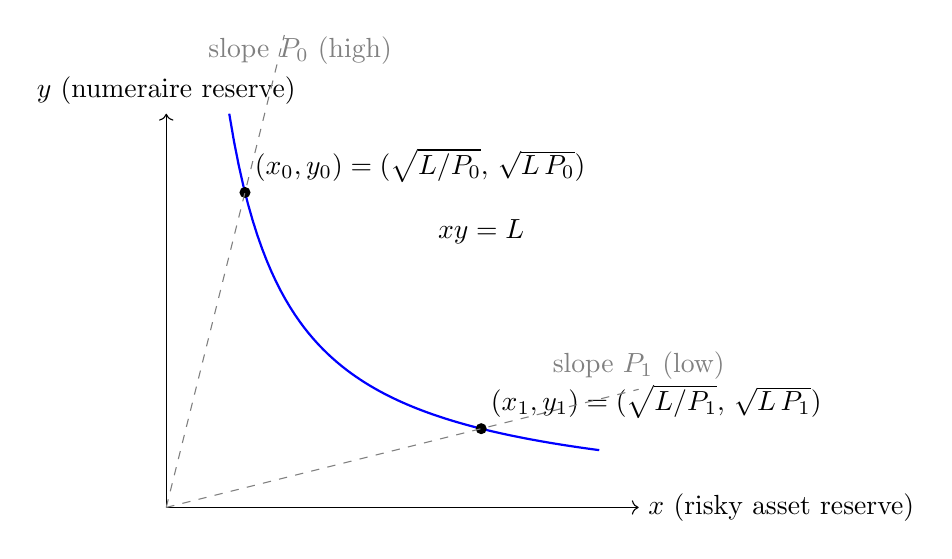
\begin{tikzpicture}[scale=1.0]
  % Axes
  \draw[->] (0,0) -- (6,0) node[right] {$x$ (risky asset reserve)};
  \draw[->] (0,0) -- (0,5) node[above] {$y$ (numeraire reserve)};
  % Hyperbola xy = 4
  \draw[thick, blue, domain=0.8:5.5, samples=80] plot (\x, {4/\x});
  % Two example points
  \fill (1.0,4.0) circle (2pt);
  \node[above right] at (1.0,4.0) {$(x_0, y_0) = (\sqrt{L/P_0},\,\sqrt{L\,P_0})$};
  \fill (4.0,1.0) circle (2pt);
  \node[above right] at (4.0,1.0) {$(x_1, y_1) = (\sqrt{L/P_1},\,\sqrt{L\,P_1})$};
  % Slope-line annotations (rays from origin)
  \draw[gray, dashed, thin] (0,0) -- (1.5,6);
  \draw[gray, dashed, thin] (0,0) -- (6,1.5);
  \node[gray] at (1.7, 5.8) {slope $P_0$ (high)};
  \node[gray] at (6, 1.8) {slope $P_1$ (low)};
  % Curve label
  \node at (4.0, 3.5) {$xy = L$};
\end{tikzpicture}
\caption{The constant-product invariant $xy = L$ in reserve space. As trades happen, the pool moves along the blue hyperbola. The marginal price $P = y/x$ is the slope of the line from the origin to the current reserve point. A high $P$ puts the pool in the upper-left of the curve (much numeraire, little risky asset). A low $P$ puts it in the lower-right.}
\label{fig:invariant}
\end{figure}

\paragraph{Pool value.}
The total value of the pool, expressed in units of the numeraire, when the marginal price is $P$ is
\[
V(P) \;:=\; y(P) + P\,x(P) \;=\; \sqrt{LP} + P\sqrt{L/P}.
\]
The second term simplifies: $P\sqrt{L/P} = \sqrt{P^2 \cdot L/P} = \sqrt{LP}$. So
\begin{equation}\label{eq:V}
\boxed{V(P) \;=\; 2\sqrt{LP}.}
\end{equation}
This is the function whose curvature drives every LVR calculation that follows.

\begin{figure}[h]
\centering
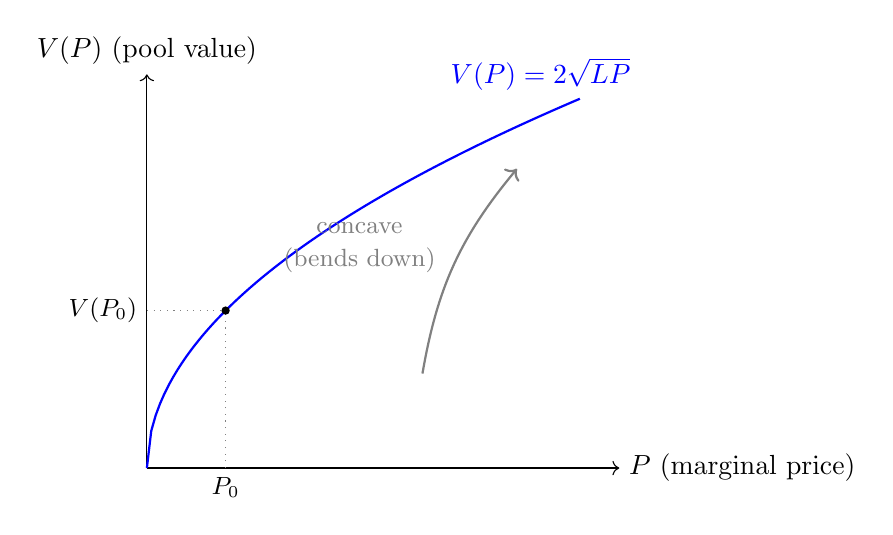
\begin{tikzpicture}[scale=1.0]
  % Axes
  \draw[->] (0,0) -- (6,0) node[right] {$P$ (marginal price)};
  \draw[->] (0,0) -- (0,5) node[above] {$V(P)$ (pool value)};
  % V(P) = 2*sqrt(P) (with L = 1)
  \draw[thick, blue, domain=0:5.5, samples=100] plot (\x, {2*sqrt(\x)});
  % Annotate curve
  \node[blue] at (5, 5) {$V(P) = 2\sqrt{LP}$};
  % Mark a few key features
  \draw[gray, dotted] (1,0) -- (1,2);
  \draw[gray, dotted] (0,2) -- (1,2);
  \fill (1,2) circle (1.5pt);
  \node[below] at (1,0) {\small $P_0$};
  \node[left] at (0,2) {\small $V(P_0)$};
  % Concavity arrow
  \draw[->, gray, thick] (3.5,1.2) to[bend left=15] (4.7,3.8);
  \node[gray, align=center] at (2.7, 2.8) {\small concave \\ \small (bends down)};
\end{tikzpicture}
\caption{The pool value $V(P) = 2\sqrt{LP}$ as a function of the marginal price. $V$ is increasing (a higher price means a more valuable pool) and concave (the curve bends down). The concavity is what costs the LP: a continuously-rebalanced portfolio with the same marginal exposure as the pool would follow the tangent line, which always sits above the curve. The gap between tangent and curve is LVR.}
\label{fig:Vcurve}
\end{figure}

\paragraph{The envelope identity.}
Differentiate $V$ with respect to $P$:
\[
V'(P) \;=\; \frac{d}{dP}\,2\sqrt{LP} \;=\; 2 \cdot \frac{1}{2} \cdot \frac{L}{\sqrt{LP}} \;=\; \frac{\sqrt{L}}{\sqrt{P}} \;=\; \sqrt{L/P}.
\]
But $\sqrt{L/P} = x(P)$. So
\begin{equation}\label{eq:envelope}
\boxed{V'(P) \;=\; x(P).}
\end{equation}
This is called the \emph{envelope identity}: the marginal change in pool value with respect to price equals the risky-asset holding. It is a deep fact about all constant-function market makers, not just constant-product.

Why does it hold? Intuitively, when the price moves by $\Delta P$, two things change. (i) The pool still holds $x(P)$ units of risky asset at the moment of the move, and that holding contributes a change $x(P) \cdot \Delta P$ to the pool value (mark-to-market on existing inventory). (ii) The pool will also rebalance: $x$ and $y$ shift along the invariant curve $xy = L$ to keep the marginal price equal to the new $P + \Delta P$. But this second effect, by the envelope theorem from constrained optimization, has zero first-order contribution at the constrained optimum. So only the first effect matters at leading order, giving $V'(P) = x(P)$.

\paragraph{Concavity.}
Differentiate once more:
\[
V''(P) \;=\; \frac{d}{dP}\,\sqrt{L}\,P^{-1/2} \;=\; -\frac{1}{2}\sqrt{L}\,P^{-3/2} \;=\; -\frac{x(P)}{2P}.
\]
Since $x(P) > 0$ and $P > 0$, we have $V''(P) < 0$ everywhere: $V$ is \emph{concave} in $P$.

\paragraph{Why concavity is the source of LVR.}
Concavity means that for any two prices $P_0$ and $P_1$:
\[
V(P_1) \;<\; V(P_0) + V'(P_0) \cdot (P_1 - P_0).
\]
The right-hand side is the tangent line to $V$ at $P_0$, evaluated at $P_1$. So the pool value sits \emph{below} the tangent line.

Operationally: imagine the price moves from $P_0$ to $P_1$. Two strategies are possible.
\begin{itemize}[leftmargin=2em]
\item \textbf{Bonding-curve LP (the AMM):} value goes from $V(P_0)$ to $V(P_1)$.
\item \textbf{Rebalancing-strategy LP:} hold exactly $x(P_0)$ units of risky asset throughout (matching the AMM's marginal exposure at the start), value goes from $V(P_0) = y(P_0) + P_0 x(P_0)$ to $y(P_0) + P_1 x(P_0) = V(P_0) + x(P_0)(P_1 - P_0)$.
\end{itemize}
The gap between the rebalancing-strategy value and the AMM value is the area between the tangent line and the curve. By concavity, this gap is non-negative and grows quadratically in $|P_1 - P_0|$. \emph{That gap is the LVR.}

\begin{figure}[h]
\centering
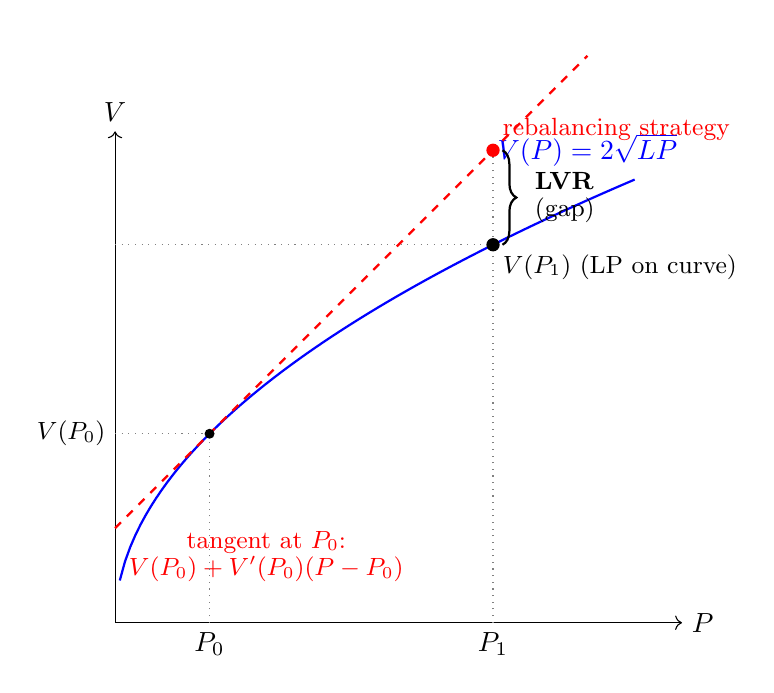
\begin{tikzpicture}[scale=1.2]
  % Axes
  \draw[->] (0,0) -- (6,0) node[right] {$P$};
  \draw[->] (0,0) -- (0,5.2) node[above] {$V$};
  % V(P) = 2 sqrt(P), L = 1
  \draw[thick, blue, domain=0.05:5.5, samples=100] plot (\x, {2*sqrt(\x)});
  \node[blue] at (5.0, 5.0) {$V(P) = 2\sqrt{LP}$};
  % P_0 = 1, V(P_0) = 2, V'(P_0) = 1
  \def\Pzero{1.0}
  \def\Vzero{2.0}
  \def\dVzero{1.0}
  % Tangent line: y = V(P_0) + V'(P_0)(x - P_0)
  \draw[thick, red, dashed, domain=0:5] plot (\x, {\Vzero + \dVzero*(\x - \Pzero)});
  \node[red] at (5.0, 6.2) {};
  \node[red, align=center] at (1.6, 0.7) {\small tangent at $P_0$: \\[-2pt] \small $V(P_0) + V'(P_0)(P - P_0)$};
  % P_1 = 4, V(P_1) = 4, tangent at P_1 = 5
  \def\Pone{4.0}
  \def\Vone{4.0}
  \def\Ttwo{5.0}
  % Vertical lines
  \draw[gray, dotted] (\Pzero,0) -- (\Pzero,\Vzero);
  \draw[gray, dotted] (\Pone,0) -- (\Pone,\Ttwo);
  \draw[gray, dotted] (0,\Vzero) -- (\Pzero,\Vzero);
  \draw[gray, dotted] (0,\Vone) -- (\Pone,\Vone);
  % Labels on x-axis
  \node[below] at (\Pzero,0) {$P_0$};
  \node[below] at (\Pone,0) {$P_1$};
  \node[left] at (0,\Vzero) {\small $V(P_0)$};
  % Dots
  \fill (\Pzero,\Vzero) circle (1.5pt);
  \fill (\Pone,\Vone) circle (2pt);
  \fill[red] (\Pone,\Ttwo) circle (2pt);
  % Brace showing LVR
  \draw[decorate, decoration={brace, amplitude=5pt, mirror}, thick]
    (\Pone+0.1, \Vone) -- (\Pone+0.1, \Ttwo)
    node[midway, right=8pt, align=left] {\small \textbf{LVR}\\[-2pt]\small (gap)};
  % Labels for the two endpoints at P1
  \node[below right] at (\Pone, \Vone) {\small $V(P_1)$ (LP on curve)};
  \node[above right, red] at (\Pone, \Ttwo) {\small rebalancing strategy};
\end{tikzpicture}
\caption{LVR as the gap between the rebalancing strategy and the bonding curve. Start at $P_0$ with pool value $V(P_0)$. If the price moves to $P_1$, the bonding-curve LP ends at $V(P_1)$ (blue dot, on the curve). A rebalancing strategy that holds the same marginal exposure $x(P_0)$ throughout ends at $V(P_0) + x(P_0)(P_1 - P_0)$ (red dot, on the tangent line). Concavity guarantees the tangent dot lies above the curve dot. The vertical gap (brace) is the LVR for this single price move. Summing such gaps over a continuous price path, weighted by the second-order concavity, gives the LVR rate.}
\label{fig:LVR-gap}
\end{figure}

\subsection{The arbitrageur}

We model a single, risk-neutral, capital-unconstrained arbitrageur with the following behavior:
\begin{itemize}[leftmargin=2em]
\item Observes both $S_t$ (the external reference price) and $P_t$ (the pool marginal price) continuously.
\item Pays a proportional swap fee $\gamma \in [0, 1)$ on the AMM, expressed in log-price units. A swap effectively moves the pool's marginal price by a factor $e^{\pm\gamma}$ extra in the direction opposite to the trade. The pool charges the fee on either side of the trade direction.
\item Can trade only when a block arrives. \textbf{Blocks arrive as a Poisson process of rate $1/\dt$}, so $\dt$ is the \emph{mean} interblock time, not a fixed slot length. This follows Milionis et al.~\cite[\S3]{milionis2023automated}; Section~\ref{sec:schedule} works out what changes under a deterministic schedule.
\item Trades myopically whenever it is profitable~\cite[\S3]{milionis2023automated}: being competitive, it does not strategically wait for a better price.
\end{itemize}

\paragraph{Assumption: the arbitrageur sees $S_t$ continuously between blocks.}
The reference price $S$ is an off-chain venue price, so the arbitrageur's \emph{information} is continuous even though on-chain reserves settle only at block inclusion. Mempool visibility of pending transactions extends the same continuity to on-chain order flow, so the pool price is not the only price a participant can observe between blocks. What the block schedule rations is the ability to \emph{act}, not the ability to \emph{see}. This is the assumption that makes the mispricing $z_t$ of Section~\ref{sec:stationary} a continuously-evolving state that is only intermittently reset.

\paragraph{Assumption: Poisson block arrivals.}
Real proof-of-stake chains produce blocks on a deterministic slot schedule, so this is a tractability assumption, inherited from~\cite{milionis2023automated}, who describe it as ``an approximation that is necessary for tractability.'' It buys the memorylessness that makes the stationary law of Section~\ref{sec:stationary} solvable in closed form. It is not free: Section~\ref{sec:schedule} shows numerically that randomizing the slot inflates the diffusion channel by up to $21\%$, and Nezlobin and Tassy~\cite{nezlobin2025lvr} prove that among block-time distributions with a given mean, arbitrage profit is \emph{minimized} by the deterministic schedule. So the Poisson assumption is conservative in a precise sense: it overstates arbitrage profit relative to the real schedule.

\paragraph{The no-arbitrage band.}
The fee $\gamma$ creates a band of inaction. If the pool's log-price is within $\gamma$ of the external log-price, no trade is profitable: the arb's profit from rebalancing the pool would be smaller than the fee they would pay. Outside this band, the arb trades, bringing the pool just to the edge of the band.

So at block-end: either the log-discrepancy $|\log P_t - \log S_t| \le \gamma$ and the arb does nothing, or the arb trades and brings the pool to $\log P_t = \log S_t \mp \gamma$ (i.e., to distance exactly $\gamma$ from the external, on the opposite side from the direction of the move).

\paragraph{Assumption: the arbitrageur is frictionless, and what that biases.}
We assume zero latency, unlimited capital, and no order-flow-auction rebate to LPs. Each of these pushes the computed rate above the realized one: latency lets some price moves partly dissipate before the arb can act, capital limits make some arbitrage sub-optimal, and auction designs rebate part of the rent. So the rate computed here is an upper bound on realized arbitrage profit. The idealization is weakest exactly in the sub-second regime that the floor argument concerns, where latency is comparable to the block time; this is stated as a limitation in the paper's conclusion.

\paragraph{What $\ell$ is, and is not: the fee-split accounting.}
This is worth pinning down early, because it is easy to misread the rate. Milionis et al.~\cite[Thms.~3--4]{milionis2023automated} show that with fees,
\[
\underbrace{\mathrm{ARB}}_{\text{arbitrageur's profit}} \;+\; \underbrace{\mathrm{FEE}}_{\text{fee income to LPs}} \;\approx\; \underbrace{\mathrm{LVR}}_{\text{frictionless, Theorem~\ref{thm:1}}}.
\]
Fees \emph{split} the frictionless LVR between the arbitrageur and the LP; they do not reduce it. The quantity $\ell(\dt)$ computed from Section~\ref{sec:stationary} onward is the $\mathrm{ARB}$ half: LP adverse-selection loss \emph{net} of the fee income LPs receive back. This is why the fee multiplier will turn out to be a probability rather than a discount factor, and why the paper's policy conclusion is about the split rather than about the total. Section~\ref{sec:experiments} describes the numerical check that computes $\mathrm{FEE}$ directly, from fee rate times trade size, and confirms the identity without assuming it.

\subsection{The LVR definition}

The cumulative LVR over $[0, T]$ is
\begin{equation}\label{eq:lvr}
\mathrm{LVR}(T) \;:=\; \int_0^T V'(P_{s-})\,dP_s \;-\; \big[V(P_T) - V(P_0)\big].
\end{equation}

We now read the two terms carefully.

\paragraph{Second term: $V(P_T) - V(P_0)$.}
The LP's mark-to-market gain. If you deposited $V(P_0)$ worth of assets into the pool at time $0$, you can withdraw $V(P_T)$ worth at time $T$. This is the LP's realized P\&L (ignoring fees collected, which we treat separately or absorb into $\gamma$).

\paragraph{First term: $\int_0^T V'(P_{s-})\,dP_s$.}
This is the gain of a hypothetical strategy that continuously holds $V'(P_{s-}) = x(P_{s-})$ units of the risky asset. Read this carefully. The strategy's risky-asset holding is \emph{the same} as the pool's risky-asset holding at every instant (by the envelope identity). The difference is that the strategy is not stuck on the bonding curve. It just holds the marginal exposure and accumulates the gain of that exposure as the price moves, by trading frictionlessly on a continuous external market.

This is the \emph{rebalancing strategy}. It mirrors the LP's exposure at every instant but does so on a friction-free market.

\paragraph{The gap.}
$\mathrm{LVR}(T)$ measures how much the rebalancing strategy outperforms the bonding-curve LP. By the concavity argument above, this is non-negative. The LP is forced to follow the curve, while the rebalancing strategy is free to follow the tangent line. The gap accumulates as the price wanders.

\begin{figure}[h]
\centering
\begin{tikzpicture}[scale=0.9]
  % Axes
  \draw[->] (0,0) -- (10.5,0) node[right] {$P$};
  \draw[->] (0,0) -- (0,7.5) node[above] {$V$};
  % V(P) = 2 sqrt(P) curve
  \draw[thick, blue, domain=0.05:10, samples=100] plot (\x, {2*sqrt(\x)});
  \node[blue] at (8.5, 5.3) {$V(P)$};
  % Tangent segments (red dashed)
  % Tangent at P_0 = 1, slope V'(1) = 1, from x=1 to x=4
  \draw[red, dashed, thick] (1, 2) -- (4, 5);
  % Tangent at P_1 = 4, slope V'(4) = 0.5, from x=4 to x=9
  \draw[red, dashed, thick] (4, 4) -- (9, 6.5);
  % Points on curve (LP path)
  \fill[blue] (1, 2) circle (2.5pt);
  \fill[blue] (4, 4) circle (2.5pt);
  \fill[blue] (9, 6) circle (2.5pt);
  % Tangent overshoot points (rebalancing endpoints)
  \fill[red] (4, 5) circle (2pt);
  \fill[red] (9, 6.5) circle (2pt);
  % Vertical gap arrows (concavity bites)
  \draw[<->, thick, gray] (4.15, 4.05) -- (4.15, 4.95);
  \node[right, gray] at (4.2, 4.5) {\small gap$_1$};
  \draw[<->, thick, gray] (9.15, 6.05) -- (9.15, 6.45);
  \node[right, gray] at (9.2, 6.25) {\small gap$_2$};
  % Dotted vertical lines from x-axis
  \draw[gray, dotted] (1, 0) -- (1, 2);
  \draw[gray, dotted] (4, 0) -- (4, 4);
  \draw[gray, dotted] (9, 0) -- (9, 6);
  % x-axis labels
  \node[below] at (1, 0) {$P_0$};
  \node[below] at (4, 0) {$P_1$};
  \node[below] at (9, 0) {$P_T$};
  % Legend
  \node[blue] at (2.6, 1.0) {\small LP on curve};
  \node[red] at (6.8, 7.0) {\small rebalancing tangents};
  % Total LVR brace at right
  \node[align=left] at (12.5, 5.0) {\small $\mathrm{LVR}(T) =$\\[-2pt] \small gap$_1$ + gap$_2$};
\end{tikzpicture}
\caption{LVR accumulates over a price path. The price moves from $P_0$ through $P_1$ to $P_T$. After each step, the rebalancing strategy reaches a point on the local tangent line (red dots). Its gain is $V'(P_{\text{start}}) \cdot \Delta P$. The LP only reaches the curve (blue dots). The vertical gap at each step (gap$_1$ at $P_1$, gap$_2$ at $P_T$) is the concavity bite the LP eats. Cumulative LVR is the sum of these gaps over the path. In the continuous limit with infinitely many infinitesimal steps, the sum becomes the integral $\int_0^T V'(P_{s-})\,dP_s - [V(P_T) - V(P_0)]$. That is the LVR definition in equation~\eqref{eq:lvr}.}
\label{fig:LVR-path}
\end{figure}

\paragraph{Why this is the ``right'' notion of cost.}
LVR is a \emph{measure-independent} quantity. It does not depend on the probability of price moves, on the LP's risk preferences, or on a hedging strategy. It is a pure quadratic-variation cost paid by the LP for being stuck on the curve. This makes LVR a natural protocol-level adverse-selection metric, distinct from venue-specific measures like fee revenue or impermanent loss vs.\ buy-and-hold.

\paragraph{What ``measure-independent'' means precisely, and how we use it.}
A \emph{probability measure} on the space of price paths assigns a likelihood to each possible trajectory of $S_t$. The SDE~\eqref{eq:sde} specifies three pieces: drift $\mu$, volatility $\sigma$, and a jump law $(\lambda, J)$. The value of the drift $\mu$ depends on which measure you work under. Under the \emph{physical measure} (the ``real'' probabilities you observe in data) $\mu$ might be the empirical average return, e.g.\ $0.50$/yr if ETH happened to appreciate by 50\% over the sample. Under an \emph{$S$-martingale measure} (where $S_t$ has zero expected return), $\mu$ takes a different value, namely $-\lambda \E[e^J - 1]$ to compensate for the jump-induced drift. Both measures describe the same underlying process. They differ only in how they re-weight paths and hence in the value assigned to $\mu$.

The diffusion volatility $\sigma$ and the jump law $(\lambda, m, \delta)$ are \emph{invariant} under any equivalent change of measure. They describe the second-order and discontinuous structure of paths, which all measures agree on. \emph{Measure-independence of LVR} is the statement that $\ell$ depends only on these invariant pieces and not on $\mu$. This is intuitive once you see why. LVR is defined as the gap between the LP's mark-to-market and a rebalancing portfolio that holds $V'(P_{s-})$ units of the risky asset at every instant. Both the LP and the rebalancing portfolio ride the same drift identically. Whatever expected return is baked into $\mu$ shows up equally on both sides of the LVR comparison and cancels exactly. What remains is the concavity bite from $V$ being curved (the $\sigma^2$ piece) and from jumps (the $J$ piece). The proof of Theorem~1 makes this concrete. The term $\int V'(S_{s-})\,\mu S_{s-}\,ds$ from the drift appears symmetrically in the rebalancing integral and in the Itô expansion of $V(S_t)$, and the two contributions subtract to zero.

\paragraph{Where measure-independence applies, and where it stops.}
It is important to be precise about the reach of this property, because the paper uses it in one place and explicitly declines to use it in another.

\emph{At $\gamma = 0$ it is a genuine invariance.} Theorem~\ref{thm:1} is a statement about quadratic variation and jump marks only. The drift cancels between the LP and the rebalancing benchmark, exactly as described above, and $\mu$ appears nowhere in the answer. Nothing is assumed about $\mu$ to prove Theorem~\ref{thm:1}, and nothing needs to be.

\emph{At $\gamma > 0$ it stops.} Once the fee opens a no-arbitrage band, the rate stops being a pure quadratic-variation object. As Section~\ref{sec:stationary} will show, it becomes an expectation against the \emph{stationary law} of the mispricing process $z_t$, and that law does depend on the drift of $\log S$: a drift tilts the law, making one tail fatter than the other. So the drift no longer cancels.

\paragraph{Assumption (a restriction, not a normalization): $\mu = \tfrac12\sigma^2 - \lambda m$.}
Following Milionis et al.~\cite[Assumption~2]{milionis2023automated}, who set $\mu = \tfrac12\sigma^2$ in the pure-GBM case, we take
\[
\mu \;=\; \tfrac{1}{2}\sigma^2 - \lambda m ,
\]
which makes $\log S_t$ exactly driftless: the diffusion contribution $\mu - \tfrac12\sigma^2$ and the jump contribution $\lambda m$ both vanish. This makes the stationary law of $z$ symmetric and is what lets the closed forms below be written down.

Because the $\gamma>0$ rate depends on the full law of $z$ and not only on its quadratic variation, \textbf{this is a modelling restriction, not a change of measure that leaves the answer invariant.} The honest question is therefore not ``is it without loss of generality?'' (it is not) but ``how much does it cost?'' Milionis et al.~\cite[Thm.~8]{milionis2023automated} answer this: a non-zero drift $\Delta$ tilts the stationary density by the exponential factor $e^{2\Delta x/\sigma^2}$, i.e.\ by a relative amount $2\Delta\gamma/\sigma^2$ across the band. At the calibration of Section~\ref{sec:calibration} that tilt is of order $10^{-3}$ for any $|\Delta| \le 1.6$/yr, which comfortably covers the realized ETH drift over the sample, and it moves $\ell$ by under $0.01\%$. The restriction is cheap, but it is a restriction, and the paper says so in its Remark~3 rather than hiding it in a change of measure.

\paragraph{The rate.}
For the theorems we work with the instantaneous expected rate:
\begin{equation}\label{eq:rate}
\ell(t) \;:=\; \frac{\E_t[d\mathrm{LVR}_t]}{dt}.
\end{equation}
This is a number with units of numeraire per unit time, for example USDC per year if the numeraire is USDC. It depends on the price-process parameters $(\sigma, \lambda, m, \delta)$, the fee $\gamma$, the block time $\dt$, and the pool value $V(P_t)$.

The whole paper is about how $\ell$ depends on $\dt$.

\section{Theorem 1: the zero-fee LVR decomposition}\label{sec:thm1}

\subsection{Statement}

\begin{theorem}\label{thm:1}
In the continuous-arbitrage limit ($\gamma = 0$, $\dt \to 0$), the pool price $P_t$ equals the reference price $S_t$ at every instant. Then for the constant-product pool value $V(P) = 2\sqrt{LP}$ under the Merton jump-diffusion~\eqref{eq:sde}, the expected LVR rate is
\begin{equation}\label{eq:thm1}
\ell \;=\; \underbrace{\frac{\sigma^2}{8}\,V_t}_{\text{diffusion}} \;+\; \underbrace{\frac{\lambda}{2}\,V_t\,\E\!\left[(e^{J/2} - 1)^2\right]}_{\text{jump}},
\end{equation}
and for $J \sim \mathcal{N}(m, \delta^2)$,
\begin{equation}\label{eq:moment}
\E\!\left[(e^{J/2} - 1)^2\right] \;=\; e^{m + \delta^2/2} - 2 e^{m/2 + \delta^2/8} + 1 \;\ge\; 0.
\end{equation}
This expression is $0$ if and only if $J \equiv 0$.
\end{theorem}

The proof has four pieces. (i) Apply the Itô–Lévy formula to $V(S_t)$. (ii) Substitute into the LVR definition. (iii) Evaluate the diffusion term using the constant-product structure. (iv) Evaluate the jump term using the elegant algebraic identity for $V$. Then take expectations using the marked-Poisson compensator and evaluate the moment for Merton jumps.

\subsection{Step 1: the Itô–Lévy formula for $V(S_t)$}

We apply the Itô formula for jump-diffusion processes (Cont \& Tankov 2003, Proposition~8.14, page~275) to the function $V$ and the price $S$. The formula states: for a jump-diffusion $S$ with drift, Brownian, and compound-Poisson components, and a $C^{1,2}$ function $f$,
\begin{align*}
f(t, S_t) - f(0, S_0) \;=\;& \int_0^t \frac{\partial f}{\partial s}(s, S_s)\,ds \;+\; \int_0^t \frac{\partial f}{\partial x}(s, S_{s-})\,dS_s \;+\; \tfrac{1}{2}\int_0^t \frac{\partial^2 f}{\partial x^2}(s, S_{s-})\,d[S, S]^c_s \\
&+\; \sum_{0 < s \le t}\!\Big[f(s, S_s) - f(s, S_{s-}) - \Delta S_s \cdot \tfrac{\partial f}{\partial x}(s, S_{s-})\Big].
\end{align*}
(This is the semimartingale version, Prop~8.19, p.~280. It is algebraically equivalent to Prop~8.14 and matches the form we use.)

For our $V$ (no time dependence) and our jump-diffusion $S$ (so $d[S,S]^c_s = \sigma^2 S_{s-}^2\,ds$), this specializes to
\begin{align*}
V(S_t) - V(S_0) \;=\;& \int_0^t V'(S_{s-})\,dS_s \\
&+ \tfrac{1}{2}\int_0^t V''(S_{s-})\,\sigma^2 S_{s-}^2\,ds \\
&+ \sum_{0 < s \le t}\!\Big[V(S_s) - V(S_{s-}) - V'(S_{s-})\,\Delta S_s\Big].
\end{align*}

Reading this term by term:
\begin{enumerate}[leftmargin=2em]
\item \emph{The dS integral} $\int_0^t V'(S_{s-})\,dS_s$. This collects the gains of the ``rebalancing strategy'' that holds $V'(S_{s-})$ units of $S$ at every instant. It is the first term of the LVR definition.
\item \emph{The Itô correction} $\tfrac{1}{2}\int_0^t V''(S_{s-})\sigma^2 S_{s-}^2\,ds$. This is the standard ``half-times-gamma-times-vol-squared'' continuous quadratic-variation correction.
\item \emph{The jump remainder} $\sum [V(S_s) - V(S_{s-}) - V'(S_{s-})\Delta S_s]$. At each jump, this is the gap between the actual change in $V$ and the linear (tangent-line) approximation. Concavity makes this non-positive.
\end{enumerate}

Figure~\ref{fig:itolevy} visualizes the geometric content of the three terms.

\begin{figure}[h]
\centering
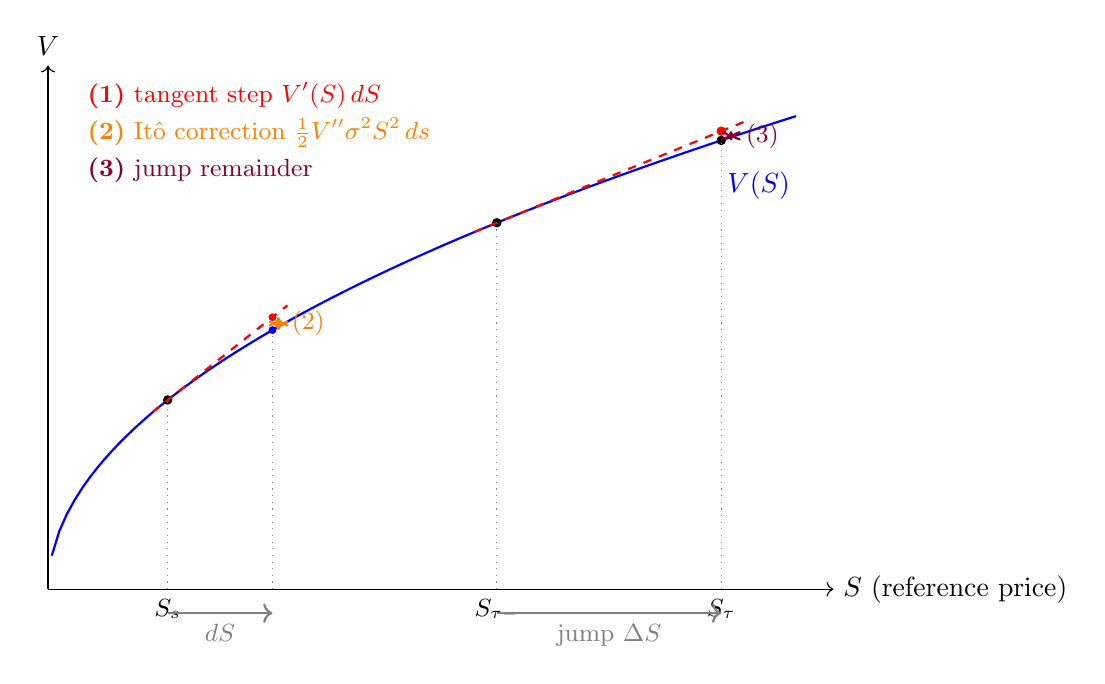
\begin{tikzpicture}[scale=0.95]
  % Axes
  \draw[->] (0,0) -- (10.5,0) node[right] {$S$ (reference price)};
  \draw[->] (0,0) -- (0,7.0) node[above] {$V$};
  % V(S) curve
  \draw[thick, blue, domain=0.05:10, samples=100] plot (\x, {2*sqrt(\x)});
  \node[blue] at (9.5, 5.4) {$V(S)$};

  %% Continuous-step zoom (left side: terms 1 and 2)
  \def\Pc{1.6}    % continuous current price
  \def\Vc{2.530}  % V(P_c) = 2 sqrt(P_c)
  \def\dVc{0.790} % V'(P_c) = 1/sqrt(P_c)
  \def\dPc{1.4}   % small dS for illustration

  % Mark point on curve, dotted vertical
  \fill (\Pc, \Vc) circle (1.8pt);
  \draw[gray, dotted] (\Pc, 0) -- (\Pc, \Vc);
  \node[below] at (\Pc, 0) {\small $S_s$};

  % dS arrow on x-axis
  \draw[->, thick, gray] (\Pc, -0.32) -- (\Pc+\dPc, -0.32);
  \node[gray, below] at (\Pc+\dPc/2, -0.34) {\small $dS$};
  \draw[gray, dotted] (\Pc+\dPc, 0) -- (\Pc+\dPc, {2*sqrt(\Pc+\dPc)});

  % Tangent at S_s, extended slightly past S_s + dS
  \draw[red, dashed, thick] (\Pc-0.2, {\Vc - \dVc*0.2}) -- (\Pc+\dPc+0.2, {\Vc + \dVc*(\dPc+0.2)});

  % Endpoint on curve and on tangent at S_s + dS
  \fill[blue] (\Pc+\dPc, {2*sqrt(\Pc+\dPc)}) circle (1.5pt);
  \fill[red] (\Pc+\dPc, {\Vc + \dVc*\dPc}) circle (1.5pt);

  % Itô correction gap brace
  \draw[<->, thick, orange] (\Pc+\dPc+0.08, {2*sqrt(\Pc+\dPc)}) -- (\Pc+\dPc+0.08, {\Vc + \dVc*\dPc});
  \node[orange, right] at (\Pc+\dPc+0.13, {(2*sqrt(\Pc+\dPc) + \Vc + \dVc*\dPc)/2}) {\small (2)};

  %% Jump (right side: term 3)
  \def\Stm{6}    % S_τ-
  \def\Vtm{4.899} % V(S_τ-) = 2 sqrt(6)
  \def\dVt{0.408} % V'(S_τ-) = 1/sqrt(6)
  \def\St{9}     % S_τ
  \def\Vt{6.0}   % V(S_τ) = 2 sqrt(9) = 6

  % Mark S_τ- and S_τ
  \fill (\Stm, \Vtm) circle (1.8pt);
  \fill (\St, \Vt) circle (1.8pt);
  \draw[gray, dotted] (\Stm, 0) -- (\Stm, \Vtm);
  \draw[gray, dotted] (\St, 0) -- (\St, \Vt);
  \node[below] at (\Stm, 0) {\small $S_{\tau-}$};
  \node[below] at (\St, 0) {\small $S_\tau$};

  % Jump arrow on x-axis
  \draw[->, thick, gray] (\Stm, -0.32) -- (\St, -0.32);
  \node[gray, below] at ({(\Stm+\St)/2}, -0.34) {\small jump $\Delta S$};

  % Tangent at S_τ-, extended to S_τ
  \draw[red, dashed, thick] (\Stm-0.3, {\Vtm - \dVt*0.3}) -- (\St+0.3, {\Vtm + \dVt*(\St-\Stm+0.3)});

  % Tangent endpoint at S_τ (red)
  \fill[red] (\St, {\Vtm + \dVt*(\St-\Stm)}) circle (1.8pt);

  % Jump-remainder brace at S_τ
  \draw[<->, thick, purple!70!black] (\St + 0.13, \Vt) -- (\St + 0.13, {\Vtm + \dVt*(\St-\Stm)});
  \node[purple!70!black, right] at (\St + 0.20, {(\Vt + \Vtm + \dVt*(\St-\Stm))/2}) {\small (3)};

  % Term labels (top-right area)
  \node[red, anchor=west] at (0.4, 6.6) {\small \textbf{(1)} tangent step $V'(S)\,dS$};
  \node[orange, anchor=west] at (0.4, 6.1) {\small \textbf{(2)} Itô correction $\tfrac{1}{2}V''\sigma^2 S^2\,ds$};
  \node[purple!70!black, anchor=west] at (0.4, 5.6) {\small \textbf{(3)} jump remainder};
\end{tikzpicture}
\caption{Geometric content of the three terms in the Itô--Lévy expansion of $V(S_t) - V(S_0)$. Along a continuous diffusive step $S_s \to S_s + dS$ (left), the rebalancing strategy gains $V'(S)\,dS$ along the tangent (red dashes, term~1). The actual curve sits below the tangent. The small vertical gap (orange) is the Itô correction $\frac{1}{2}V''(S)\sigma^2 S^2\,ds$ that accumulates as a continuous integral (term~2). At a jump $S_{\tau-} \to S_\tau$ (right), the tangent extrapolated by $\Delta S$ overshoots the curve by a finite amount. The vertical gap (purple) is the discrete \emph{jump remainder} $V(S_\tau) - V(S_{\tau-}) - V'(S_{\tau-})\Delta S$ (term~3). Both gaps are non-negative because $V$ is concave: the same mechanism, taken continuously for term~2 and discretely for term~3.}
\label{fig:itolevy}
\end{figure}

\subsection{Step 2: substitute into the LVR definition}

The LVR over $[0, t]$ is, by definition,
\[
\mathrm{LVR}(t) \;=\; \int_0^t V'(P_{s-})\,dP_s - [V(P_t) - V(P_0)].
\]
In the continuous-arbitrage limit $P_t \equiv S_t$, so this becomes
\[
\mathrm{LVR}(t) \;=\; \int_0^t V'(S_{s-})\,dS_s - [V(S_t) - V(S_0)].
\]
Substitute the Itô–Lévy expansion of $V(S_t) - V(S_0)$:
\begin{align*}
\mathrm{LVR}(t) \;=\;& \int_0^t V'(S_{s-})\,dS_s \;-\; \int_0^t V'(S_{s-})\,dS_s \\
& \;-\; \tfrac{1}{2}\int_0^t V''(S_{s-})\sigma^2 S_{s-}^2\,ds \\
& \;-\; \sum_{0 < s \le t}\big[V(S_s) - V(S_{s-}) - V'(S_{s-})\Delta S_s\big].
\end{align*}
The first two terms cancel. What remains:
\begin{equation}\label{eq:lvr-decomp}
\mathrm{LVR}(t) \;=\; -\tfrac{1}{2}\int_0^t V''(S_{s-})\,\sigma^2 S_{s-}^2\,ds \;-\; \sum_{0 < s \le t}\!\Big[V(S_s) - V(S_{s-}) - V'(S_{s-})\,\Delta S_s\Big].
\end{equation}

Both terms are non-negative:
\begin{itemize}[leftmargin=2em]
\item The integral term has $V''(S) < 0$ (concavity), so the integrand $-\tfrac{1}{2}V''\sigma^2 S^2 > 0$.
\item Each summand in the jump term: by concavity, $V(S_s) \le V(S_{s-}) + V'(S_{s-})\Delta S_s$ (the tangent line at $S_{s-}$ overestimates $V$ at the post-jump point $S_s$), so $V(S_s) - V(S_{s-}) - V'(S_{s-})\Delta S_s \le 0$, and the negative of this is $\ge 0$.
\end{itemize}

So $\mathrm{LVR}(t) \ge 0$ always. The LP always loses to (or ties with) the rebalancing strategy.

\subsection{Step 3: evaluate the diffusion term for constant-product}

We need to compute $-\tfrac{1}{2}V''(P)\sigma^2 P^2$ when $V(P) = 2\sqrt{LP}$. We computed $V''(P) = -x(P)/(2P)$ earlier. Substitute:
\[
-\tfrac{1}{2}V''(P)\sigma^2 P^2 \;=\; -\tfrac{1}{2}\cdot \Big(-\frac{x(P)}{2P}\Big)\cdot \sigma^2 P^2 \;=\; \frac{\sigma^2}{4}\,P\,x(P).
\]
Now substitute $x(P) = \sqrt{L/P}$:
\[
\frac{\sigma^2}{4}\,P \cdot \sqrt{L/P} \;=\; \frac{\sigma^2}{4}\,\sqrt{P^2 \cdot L/P} \;=\; \frac{\sigma^2}{4}\,\sqrt{LP} \;=\; \frac{\sigma^2}{4}\cdot \frac{V(P)}{2} \;=\; \frac{\sigma^2}{8}\,V(P),
\]
using $V(P) = 2\sqrt{LP}$ in the third step. So the instantaneous diffusion-LVR rate is
\begin{equation}\label{eq:diff-rate}
\ell_{\text{diff}}(P) \;=\; -\tfrac{1}{2}V''(P)\sigma^2 P^2 \;=\; \frac{\sigma^2}{8}\,V(P).
\end{equation}

This is the famous Milionis et al.\ (2022) result: for Uniswap-v2, the LVR rate under GBM is $\sigma^2 V/8$.

\subsection{Step 4: evaluate the jump remainder for constant-product}

This is the new step. At a jump time $\tau$, let $r := e^{J_\tau}$ (so $S_\tau = S_{\tau-} \cdot r$, $\Delta S_\tau = S_{\tau-}(r - 1)$).

Compute the jump-remainder bracket:
\[
V(S_\tau) - V(S_{\tau-}) - V'(S_{\tau-})\,\Delta S_\tau.
\]
Substitute $V(P) = 2\sqrt{LP}$ and $V'(P) = \sqrt{L/P}$:
\begin{align*}
V(S_{\tau-} r) &- V(S_{\tau-}) - V'(S_{\tau-}) \cdot S_{\tau-}(r-1) \\
&= 2\sqrt{L S_{\tau-} r} - 2\sqrt{L S_{\tau-}} - \sqrt{L/S_{\tau-}}\cdot S_{\tau-}(r-1).
\end{align*}
Simplify the last term: $\sqrt{L/S_{\tau-}}\cdot S_{\tau-} = \sqrt{L \cdot S_{\tau-}^2 / S_{\tau-}} = \sqrt{L S_{\tau-}}$. So
\[
V(S_{\tau-} r) - V(S_{\tau-}) - V'(S_{\tau-})\,\Delta S_\tau \;=\; 2\sqrt{L S_{\tau-} r} - 2\sqrt{L S_{\tau-}} - \sqrt{L S_{\tau-}}(r - 1).
\]
Pull out the common factor $\sqrt{L S_{\tau-}}$:
\[
= \sqrt{L S_{\tau-}}\,\big[2\sqrt{r} - 2 - (r - 1)\big] \;=\; \sqrt{L S_{\tau-}}\,\big[2\sqrt{r} - r - 1\big].
\]
The bracket simplifies elegantly. Note that
\[
(\sqrt{r} - 1)^2 \;=\; r - 2\sqrt{r} + 1.
\]
So $2\sqrt{r} - r - 1 = -(r - 2\sqrt{r} + 1) = -(\sqrt{r} - 1)^2$.

Therefore
\[
V(S_{\tau-} r) - V(S_{\tau-}) - V'(S_{\tau-})\,\Delta S_\tau \;=\; -\sqrt{L S_{\tau-}}\,(\sqrt{r} - 1)^2.
\]
Now use $\sqrt{L S_{\tau-}} = V(S_{\tau-})/2$ and $\sqrt{r} = e^{J_\tau/2}$:
\begin{equation}\label{eq:jump-loss}
\boxed{V(S_{\tau-} r) - V(S_{\tau-}) - V'(S_{\tau-})\,\Delta S_\tau \;=\; -\frac{V(S_{\tau-})}{2}\,(e^{J_\tau/2} - 1)^2.}
\end{equation}

This is the \emph{key algebraic identity}. For the constant-product pool, the jump remainder at each jump is exactly $-\tfrac{V}{2}(e^{J/2} - 1)^2$. Note the squared expression $(e^{J/2} - 1)^2$. It is symmetric in the sign of $J$, so up-jumps and down-jumps cost the LP the same amount (for a given $|J|$). And it is non-negative, as required by concavity.

\subsection{Step 5: take expected rate via the compensator}

Substituting~\eqref{eq:jump-loss} into the jump term of~\eqref{eq:lvr-decomp}:
\begin{equation}\label{eq:jump-sum}
-\sum_{0 < s \le t}\!\Big[V(S_s) - V(S_{s-}) - V'(S_{s-})\Delta S_s\Big] \;=\; \sum_{0 < s \le t} \frac{V(S_{s-})}{2}\,(e^{J_s/2} - 1)^2.
\end{equation}
The sum on the right has two random ingredients per jump: the pool value $V(S_{s-})$ just before the jump (which depends on the entire history up to time $s$) and the log-jump size $J_s$ (which is a fresh independent draw at the jump). We need the expectation of this sum, divided by $t$, to extract the rate.

The tool is the \textbf{marked-Poisson compensator formula} from Cont \& Tankov (2003, Prop.~8.8, p.~262).\footnote{Cont \& Tankov build up the compensated integral and the intensity measure $\lambda\,\nu(dy)\,ds$ in three layers. Reading them in order shows where each piece comes from. \emph{(1) The 1D compensated Poisson process} (\S2.5.4, p.~\textasciitilde80) defines $\tilde N_t = N_t - \lambda t$ as a martingale and calls $\lambda t$ the ``compensator of $N_t$.'' \emph{(2) Compensated Poisson random measure} (\S2.6.1, Def.~2.18, p.~\textasciitilde85, and \S2.6.2, p.~\textasciitilde88) generalizes (1) from a 1D process to a random measure $M$ on $\R^d$, defining $\tilde M(A) = M(A) - \mu(A)$ where $\mu$ is the intensity measure. \emph{(3) Compound-Poisson factorization} (\S3.2, Prop.~3.5, p.~\textasciitilde75) shows that for a compound Poisson process with rate $\lambda$ and jump-size law $\nu$, the intensity measure factorizes as $\mu(dy\,ds) = \lambda\,\nu(dy)\,ds$. This is the specific form we use. \emph{(4) Stochastic integration against $\tilde M$} (\S8.1.4). Prop.~8.7 (p.~\textasciitilde261) gives the martingale property for simple predictable integrands. Prop.~8.8 (p.~262) is the $L^2$ extension that we cite. The compensator formula $\E[\int\!\int\phi\,dM] = \E[\int\!\int\phi\,d\mu]$ is an immediate corollary of $\E[\int\!\int\phi\,d\tilde M] = 0$.} The next few paragraphs walk through how the formula applies, step by step.

\paragraph{Step 5a: rewrite the sum as a random-measure integral.}
Recall from Section~\ref{sec:setup} that the random measure $J(ds, dy)$ places a unit point mass at each $(\tau_i, J_{\tau_i})$. That is one mass for each (jump time, log-jump size) pair. Integrals against $J$ are pathwise sums:
\[
\int_0^t \!\int_\R \phi(s, y)\,J(ds, dy) \;=\; \sum_{\tau_i \le t} \phi(\tau_i, J_{\tau_i}).
\]
Our sum~\eqref{eq:jump-sum} fits this pattern with the integrand
\[
\phi(s, y) \;:=\; \frac{V(S_{s-})}{2}\,(e^{y/2} - 1)^2.
\]
So
\begin{equation}\label{eq:sum-as-integral}
\sum_{0 < s \le t} \frac{V(S_{s-})}{2}\,(e^{J_s/2} - 1)^2 \;=\; \int_0^t\!\int_\R \frac{V(S_{s-})}{2}\,(e^{y/2} - 1)^2\,J(ds, dy).
\end{equation}
This is just a notational change. The right-hand side packages the sum as an integral against the random measure. The point is to put the expression in the form the Cont--Tankov machinery is built for.

\paragraph{Step 5b: state Prop 8.8 precisely.}
The formal content of Proposition~8.8 (page~262 of Cont \& Tankov) is that for any \emph{predictable} integrand $\phi: \Omega \times [0,T] \times \R \to \R$ satisfying the square-integrability condition $\E[\int_0^t\!\int |\phi(s,y)|^2 \lambda\,\nu(dy)\,ds] < \infty$, the \emph{compensated integral}
\[
M_t \;:=\; \int_0^t\!\int_\R \phi(s, y)\,\big(J(ds, dy) - \lambda\,\nu(dy)\,ds\big)
\]
is a square-integrable martingale with mean zero. The deterministic measure $\lambda\,\nu(dy)\,ds$ that is subtracted from $J(ds, dy)$ is the \emph{compensator}: it is what is needed to subtract out the systematic part of $J$ and leave a pure noise term.

The corollary we want, the so-called \emph{compensator formula}, is immediate from $\E[M_t] = 0$:
\begin{equation}\label{eq:compensator}
\E\!\left[\int_0^t\!\int_\R \phi(s, y)\,J(ds, dy)\right] \;=\; \E\!\left[\int_0^t\!\int_\R \phi(s, y)\,\lambda\,\nu(dy)\,ds\right].
\end{equation}
In words: \emph{the expected integral of $\phi$ against the random measure equals the integral of $\phi$ against the deterministic intensity measure.} The randomness of $J$ has been ``averaged out'' against the deterministic compensator.

\paragraph{Step 5c: verify the integrand is predictable.}
The compensator formula requires $\phi(s, y)$ to be \emph{predictable}. Informally, that means ``determined by what happened up to and excluding time $s$.'' Our integrand decomposes as
\[
\phi(s, y) \;=\; \underbrace{\frac{V(S_{s-})}{2}}_{\mathcal{F}_{s-}\text{-measurable}} \;\cdot\; \underbrace{(e^{y/2} - 1)^2}_{\text{deterministic in }y}.
\]
The first factor $V(S_{s-})$ is $\mathcal{F}_{s-}$-measurable (it depends only on the price history strictly before $s$, since $S_{s-}$ is the left-limit). The second factor is a fixed deterministic function of the mark $y$. So $\phi$ is jointly predictable in $(s, y)$, and the integrability condition is easily satisfied for bounded $V$ over $[0, t]$. Prop~8.8 applies.

\paragraph{Step 5d: apply the compensator formula and split the integral.}
Plug~\eqref{eq:sum-as-integral} into~\eqref{eq:compensator}:
\[
\E\!\left[\sum_{0 < s \le t} \frac{V(S_{s-})}{2}\,(e^{J_s/2} - 1)^2\right] \;=\; \E\!\left[\int_0^t\!\int_\R \frac{V(S_{s-})}{2}\,(e^{y/2} - 1)^2\,\lambda\,\nu(dy)\,ds\right].
\]
Now we can split the inner $y$-integral from the outer $s$-integral, because the integrand factorizes:
\begin{align*}
\E\!\left[\int_0^t\!\int_\R \frac{V(S_{s-})}{2}\,(e^{y/2} - 1)^2\,\lambda\,\nu(dy)\,ds\right]
&\;=\; \lambda\,\E\!\left[\int_0^t \frac{V(S_{s-})}{2}\,\left(\int_\R (e^{y/2} - 1)^2\,\nu(dy)\right)\!ds\right] \\
&\;=\; \lambda \cdot \underbrace{\int_\R (e^{y/2} - 1)^2\,\nu(dy)}_{=\,\E[(e^{J/2} - 1)^2]} \cdot \tfrac{1}{2}\,\E\!\left[\int_0^t V(S_{s-})\,ds\right].
\end{align*}
In the second line: the $y$-integral does not depend on $\omega$ or on $s$, so it pulls out of both the $s$-integral and the expectation. And $\int_\R (e^{y/2} - 1)^2\,\nu(dy)$ is exactly the moment $\E[(e^{J/2} - 1)^2]$ (by definition of $\nu$ as the distribution of $J$). The remaining factor $\E[\int_0^t V(S_{s-})\,ds]$ collects the expected time-integral of the pool value over the interval $[0, t]$.

Putting it together:
\begin{equation}\label{eq:compensator-applied}
\E\!\left[\sum_{0 < s \le t} \frac{V(S_{s-})}{2}\,(e^{J_s/2} - 1)^2\right] \;=\; \frac{\lambda}{2}\,\E[(e^{J/2} - 1)^2]\,\cdot\,\E\!\left[\int_0^t V(S_{s-})\,ds\right].
\end{equation}

\paragraph{Step 5e: extract the rate.}
Equation~\eqref{eq:compensator-applied} gives the cumulative expected jump-LVR over $[0, t]$. To get the instantaneous rate, we differentiate both sides with respect to $t$ and then condition on the present state. There are three substeps. Each one is small but worth making explicit, because the result $V_t$ (not $\E[V_t]$) sits a bit subtly.

\emph{First, the Fundamental Theorem of Calculus.} For every sample path, $\int_0^t V(S_{s-})\,ds$ is an ordinary Lebesgue integral with upper limit $t$, and
\[
\frac{d}{dt}\int_0^t V(S_{s-})\,ds \;=\; V(S_{t-}) \;=\; V_t.
\]
Pathwise, the derivative at the upper limit is just the integrand evaluated at $t$.

\emph{Second, move the derivative inside the expectation.} Under the standard regularity (Leibniz / dominated convergence, which holds for any process with $\E[V(S_t)] < \infty$ at each $t$),
\[
\frac{d}{dt}\,\E\!\left[\int_0^t V(S_{s-})\,ds\right] \;=\; \E\!\left[\frac{d}{dt}\int_0^t V(S_{s-})\,ds\right] \;=\; \E[V_t].
\]
At this stage we have the \emph{unconditional} rate $\frac{\lambda}{2}\,\E[V_t]\,\E[(e^{J/2}-1)^2]$. It is still an expectation over $V_t$.

\emph{Third, condition on the present state.} The instantaneous rate we actually want is not the unconditional one. It is the \emph{conditional} rate given the history up to time $t$.
\[
\ell_{\text{jump}}(t) \;:=\; \lim_{h \to 0}\,\frac{\E_t[\mathrm{LVR}^{\text{jump}}(t+h) - \mathrm{LVR}^{\text{jump}}(t)]}{h}, \qquad \E_t[\cdot] := \E[\cdot \mid \mathcal{F}_t].
\]
Conditioning on $\mathcal{F}_t$ makes $V_t$ a known number (it is $\mathcal{F}_t$-measurable), so $\E_t[V_t] = V_t$ with no outer expectation. Over a small window $[t, t+h]$, the conditional expectation of the integral is $\E_t[\int_t^{t+h} V(S_{s-})\,ds] = V_t \cdot h + O(h^2)$, and dividing by $h$ leaves the leading coefficient $V_t$.

By contrast, the jump-mark $J$ is \emph{not} $\mathcal{F}_t$-measurable. It is a fresh draw at the next jump, independent of the history. So the inner expectation $\E[(e^{J/2}-1)^2]$ persists.

Putting the three substeps together:
\begin{equation}\label{eq:jump-rate}
\ell_{\text{jump}}(t) \;=\; \frac{\lambda}{2}\,V_t\,\E\!\left[(e^{J/2} - 1)^2\right].
\end{equation}
This is the rate \emph{at the current pool state $V_t$}, not an unconditional average over all possible $V_t$. The state-dependence is consistent with the Markov structure of $S$. Given the current value of $S_t$, the future evolution depends only on $V(S_t) = V_t$, not on the path history. It is also the natural form for the numerical illustration in Section~\ref{sec:calibration}, where $V$ is fixed at the calibration value and $\ell$ is read off as a function of that fixed state.

\paragraph{What the formula is doing, in one sentence.}
The expected sum over jumps $\sum \phi(\tau_i, J_{\tau_i})$ equals $\lambda$ times the expected time-integral of the $\nu$-average $\int \phi(s, y)\,\nu(dy)$. This is a Poisson sum factored into ``how often jumps happen'' ($\lambda$) times ``what they typically cost'' ($\int \phi\,d\nu$). For our integrand, ``how often'' is $\lambda$, ``what they typically cost'' is $\frac{V}{2}\E[(e^{J/2}-1)^2]$, and the rate is the product.

\subsection{Step 6: evaluate the moment for Merton jumps}

For $J \sim \mathcal{N}(m, \delta^2)$:
\[
\E[e^{aJ}] \;=\; e^{am + a^2 \delta^2 / 2}
\]
is the moment generating function. Expand:
\[
\E[(e^{J/2} - 1)^2] \;=\; \E[e^J - 2 e^{J/2} + 1] \;=\; \E[e^J] - 2\E[e^{J/2}] + 1.
\]
Apply the MGF at $a = 1$ and $a = 1/2$:
\[
\E[e^J] \;=\; e^{m + \delta^2 / 2}, \qquad \E[e^{J/2}] \;=\; e^{m/2 + \delta^2 / 8}.
\]
So
\begin{equation}\label{eq:merton-moment}
\E[(e^{J/2} - 1)^2] \;=\; e^{m + \delta^2 / 2} - 2 e^{m/2 + \delta^2 / 8} + 1.
\end{equation}
This is non-negative: $(e^{J/2} - 1)^2 \ge 0$ pathwise, so its expectation is $\ge 0$. (Or: by Jensen's inequality applied to the strictly convex map $u \mapsto (e^{u/2} - 1)^2$.) Equality holds only at the degenerate $J \equiv 0$.

For small $\delta$ (the regime of empirical relevance), expand to leading order:
\[
e^{m + \delta^2/2} \approx 1 + m + m^2/2 + \delta^2/2, \quad
e^{m/2 + \delta^2/8} \approx 1 + m/2 + m^2/8 + \delta^2/8,
\]
so
\[
\E[(e^{J/2}-1)^2] \;\approx\; (1 + m + m^2/2 + \delta^2/2) - 2(1 + m/2 + m^2/8 + \delta^2/8) + 1 \;=\; \frac{m^2}{4} + \frac{\delta^2}{4}.
\]
For symmetric ($m = 0$) Merton jumps: $\E[(e^{J/2}-1)^2] \approx \delta^2/4$.

\subsection{Putting it all together}

Adding the diffusion rate~\eqref{eq:diff-rate} and the jump rate~\eqref{eq:jump-rate} gives Theorem~1:
\[
\ell \;=\; \frac{\sigma^2}{8}\,V_t \;+\; \frac{\lambda}{2}\,V_t\,\E[(e^{J/2} - 1)^2] \;=\; \frac{\sigma^2}{8}\,V_t \;+\; \frac{\lambda}{2}\,V_t\,\big[e^{m + \delta^2/2} - 2 e^{m/2 + \delta^2/8} + 1\big].
\]


\section{The mispricing process and its stationary law}\label{sec:stationary}

Theorem~\ref{thm:1} is a zero-fee result: at $\gamma = 0$ the pool tracks the reference price exactly, $P_t \equiv S_t$, and there is nothing to keep track of. Everything from here on turns on what happens when $\gamma > 0$ and the pool is allowed to drift away from the reference between blocks. The object that carries all of it is the \emph{log mispricing}
\begin{equation}\label{eq:zdef}
z_t \;:=\; \log\frac{S_t}{P_t}.
\end{equation}

This section derives the law of $z$. It is the longest section of the companion, and deliberately so: the central correction relative to a naive treatment lives here, and the two theorems that follow are each one line of algebra once the law is in hand.

\subsection{Mispricing is a persistent state, not a fresh draw}

Here is the single most important structural fact in the paper, and the one that is easiest to get wrong.

Between blocks, the pool price $P$ is \emph{frozen}: nobody can trade, so the reserves cannot move. The reference price $S$, however, keeps moving. So between blocks $z$ inherits the full dynamics of $\log S$.

At a block arrival $\tau_i$, the arbitrageur looks at $z_{\tau_i^-}$ and acts:
\begin{itemize}[leftmargin=2em]
\item If $|z_{\tau_i^-}| \le \gamma$, no trade is profitable and \textbf{nothing happens}. The mispricing is carried forward untouched.
\item If $|z_{\tau_i^-}| > \gamma$, the arbitrageur trades, but only up to the edge of the band: pushing further would cost more in fees than it earns. The pool ends at log-distance exactly $\gamma$ from the reference, so
\[
z_{\tau_i} \;=\; \sgn(z_{\tau_i^-})\cdot\gamma \;=\; \bound\big(z_{\tau_i^-},\,-\gamma,\,\gamma\big).
\]
\end{itemize}
The clipping map $\bound(\cdot,-\gamma,\gamma)$ is exactly the one in Milionis et al.~\cite[Eqs.~(7)--(9)]{milionis2023automated}.

\paragraph{The trap.} Read the second bullet again. \textbf{A trade leaves $z$ at $\pm\gamma$, not at $0$.} And by the first bullet, if no trade occurs, whatever mispricing existed is still there at the start of the next interval. Put together: $z$ is a \emph{persistent state} with memory. It is never reset to zero, at any block, ever.

It is very tempting --- and it is wrong --- to model the pre-block mispricing as the diffusive increment accumulated over one block, $X \sim \mathcal N(0,\sigma^2\dt)$, as though each block re-pegged the pool to the reference. That would be the ``reset-to-zero'' model. Section~\ref{sec:resettrap} works out exactly what it costs, and the answer is: at Solana's block time, a factor of $4\times10^7$. The whole of the present section exists to avoid that error.

\subsection{The two point processes}

Applying the It\^o--L\'evy formula \cite[Prop.~8.14]{cont2003financial} to $\log S$ under the price SDE~\eqref{eq:sde}, and adding the arbitrage resets, gives the paper's Eq.~(11). Writing $\mathcal J_i := \bound(z_{\tau_i^-},-\gamma,\gamma) - z_{\tau_i^-}$ for the reset at block $i$, and $T_k$ for the jump times of $N$,
\begin{equation}\label{eq:ourz}
\boxed{\;z_t \;=\; \big(\mu - \tfrac12\sigma^2\big)t \;+\; \sigma W_t \;+\; \underbrace{\sum_{k:\,T_k \le t} J_k}_{\text{exogenous, rate }\lambda} \;+\; \underbrace{\sum_{i:\,\tau_i \le t} \mathcal J_i}_{\text{endogenous, rate }1/\dt}. \;}
\end{equation}
Under the drift restriction $\mu = \tfrac12\sigma^2 - \lambda m$ the first term vanishes.

Equation~\eqref{eq:ourz} is worth staring at, because the entire paper is a consequence of its shape. The mispricing is driven by \emph{two} point processes with opposite jobs:
\begin{itemize}[leftmargin=2em]
\item the \textbf{price jumps} $J_k$, arriving at rate $\lambda$, whose marks push $z$ \emph{away} from the band --- and whose rate the protocol does not choose;
\item the \textbf{block resets} $\mathcal J_i$, arriving at rate $1/\dt$, whose marks always push $z$ \emph{towards} the band --- and whose rate is exactly the policy variable.
\end{itemize}
This is precisely where the model departs from Milionis et al. Under a GBM reference price their mispricing~\cite[Eq.~(9)]{milionis2023automated} is a regulated Brownian motion driven by \emph{one} point process, the blocks, and every mark pushes inward. Speeding up that single process drives the mispricing to zero, which is the standard argument for short blocks. Adding a second, outward-pushing process that the protocol cannot speed up is the whole of the difference, and the floor of Section~\ref{sec:thm2} is its consequence.

\begin{figure}[h]
\centering
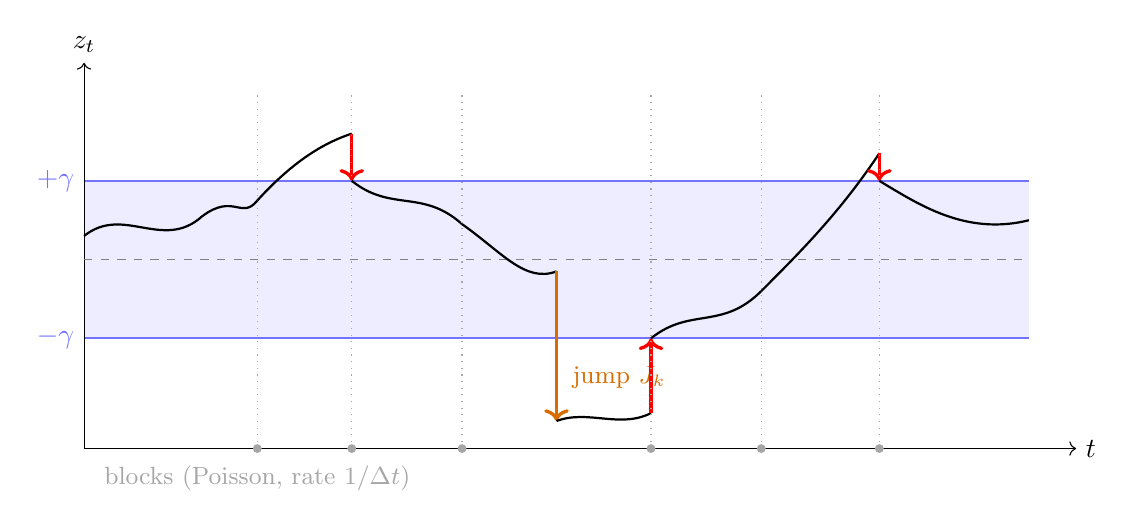
\begin{tikzpicture}[scale=1.0]
  \def\g{1.0}
  % band
  \fill[blue!7] (0,-\g) rectangle (12,\g);
  \draw[blue!55, thick] (0,\g) -- (12,\g);
  \draw[blue!55, thick] (0,-\g) -- (12,-\g);
  \node[blue!55, left] at (0,\g) {$+\gamma$};
  \node[blue!55, left] at (0,-\g) {$-\gamma$};
  % axes
  \draw[->] (0,-2.4) -- (12.6,-2.4) node[right] {$t$};
  \draw[->] (0,-2.4) -- (0,2.5) node[above] {$z_t$};
  \draw[gray, dashed, thin] (0,0) -- (12,0);
  % path: piecewise wiggly, with clips at blocks and one jump
  % segment 1: 0 -> block at 2.2, stays inside band
  \draw[thick] (0,0.3) .. controls (0.5,0.7) and (1.0,0.1) .. (1.5,0.55)
                        .. controls (1.9,0.85) and (2.0,0.5) .. (2.2,0.75);
  % block 1 at t=2.2: inside band, NO trade -> continuous
  \draw[thick] (2.2,0.75) .. controls (2.7,1.3) and (3.1,1.5) .. (3.4,1.6);
  % block 2 at t=3.4: outside band -> clip down to +gamma
  \draw[red, very thick, ->] (3.4,1.6) -- (3.4,\g);
  \draw[thick] (3.4,\g) .. controls (3.9,0.6) and (4.3,0.9) .. (4.8,0.45);
  % block 3 at t=4.8: inside -> nothing
  \draw[thick] (4.8,0.45) .. controls (5.3,0.1) and (5.6,-0.3) .. (6.0,-0.15);
  % JUMP at t=6.0
  \draw[orange!85!black, very thick, ->] (6.0,-0.15) -- (6.0,-2.05);
  \node[orange!85!black, right, font=\small] at (6.08,-1.5) {jump $J_k$};
  \draw[thick] (6.0,-2.05) .. controls (6.4,-1.9) and (6.8,-2.15) .. (7.2,-1.95);
  % block 4 at 7.2: far outside -> clip up to -gamma
  \draw[red, very thick, ->] (7.2,-1.95) -- (7.2,-\g);
  \draw[thick] (7.2,-\g) .. controls (7.7,-0.6) and (8.1,-0.9) .. (8.6,-0.4);
  % block 5 at 8.6 inside
  \draw[thick] (8.6,-0.4) .. controls (9.1,0.1) and (9.6,0.6) .. (10.1,1.35);
  % block 6 at 10.1 outside -> clip
  \draw[red, very thick, ->] (10.1,1.35) -- (10.1,\g);
  \draw[thick] (10.1,\g) .. controls (10.6,0.7) and (11.2,0.3) .. (12,0.5);
  % block markers
  \foreach \x in {2.2,3.4,4.8,7.2,8.6,10.1}{
    \draw[gray!70, dotted] (\x,-2.4) -- (\x,2.1);
    \fill[gray!70] (\x,-2.4) circle (1.6pt);
  }
  \node[gray!70, below, font=\small] at (2.2,-2.5) {blocks (Poisson, rate $1/\dt$)};
\end{tikzpicture}
\caption{One path of the mispricing $z_t$. Between blocks $z$ diffuses freely (the pool price is frozen, the reference price is not). At a block arrival (grey dotted lines) one of two things happens: if $z$ is inside the band $[-\gamma,\gamma]$ nothing happens at all and the mispricing is carried forward; if $z$ is outside, the arbitrageur trades and clips $z$ back to the \emph{near edge} $\pm\gamma$ (red arrows) --- \emph{not} to zero. A price jump (orange) throws $z$ far outside the band in one instant, at a rate the protocol does not control; it is cleared at the next block whatever the block rate is. The two kinds of arrow are the two point processes in~\eqref{eq:ourz}, and they push in opposite directions.}
\label{fig:zpath}
\end{figure}

\subsection{The stationary law: statement}

Set $\lambda = 0$ for the moment (pure diffusion, no jumps); the jump channel is added back in Section~\ref{sec:G} and the error from treating them separately is bounded in Section~\ref{sec:prop1}. Write $\beta := 1/\dt$ for the block rate and define
\begin{equation}\label{eq:theta}
\theta \;:=\; \frac{\sqrt{2\beta}}{\sigma} \;=\; \frac{\sqrt{2/\dt}}{\sigma},
\qquad
\eta \;:=\; \theta\gamma \;=\; \frac{\sqrt2\,\gamma}{\sigma\sqrt{\dt}} \;=\; \sqrt2\,\kappa .
\end{equation}

\begin{lemma}[Stationary mispricing; Milionis et al.~\cite{milionis2023automated}, Thm.~1]\label{lem:pi}
For $\lambda = 0$ the process $z$ is ergodic with stationary density
\begin{equation}\label{eq:pi0}
p(x) \;=\;
\begin{cases}
c, & |x| \le \gamma,\\[2pt]
c\,e^{-\theta(|x|-\gamma)}, & |x| > \gamma,
\end{cases}
\qquad c \;=\; \frac{\theta}{2(1+\eta)} .
\end{equation}
It is \textbf{uniform on the no-arbitrage band}, carrying mass $\eta/(1+\eta)$ there, with \textbf{exponential tails} outside carrying mass $\tfrac12(1+\eta)^{-1}$ each. In particular
\begin{equation}\label{eq:ptrade}
\Prob_\pi\big(|z| > \gamma\big) \;=\; \frac{1}{1+\eta} .
\end{equation}
\end{lemma}

Before verifying this, note the shape: a flat slab over the band with two exponential shoulders. Figure~\ref{fig:pi} draws it at three block times.

\begin{figure}[h]
\centering
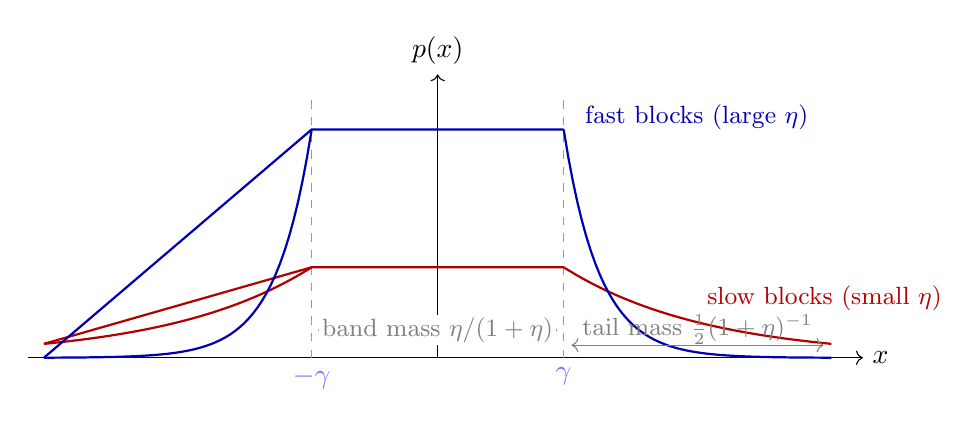
\begin{tikzpicture}[scale=1.0]
  \def\g{1.6}
  \draw[->] (-5.2,0) -- (5.4,0) node[right] {$x$};
  \draw[->] (0,0) -- (0,3.6) node[above] {$p(x)$};
  \draw[blue!45, dashed] (-\g,0) -- (-\g,3.3);
  \draw[blue!45, dashed] (\g,0) -- (\g,3.3);
  \node[blue!55, below] at (\g,0) {$\gamma$};
  \node[blue!55, below] at (-\g,0) {$-\gamma$};
  % slow blocks: small theta -> low slab, wide tails.  theta1 = 0.55, c1 = 0.55/(2(1+0.88)) scaled
  \draw[thick, red!70!black] (-5.0,{1.15*exp(-0.55*(5.0-\g))}) -- (-\g,1.15) -- (\g,1.15)
        plot[domain=\g:5.0, samples=60] (\x, {1.15*exp(-0.55*(\x-\g))});
  \draw[thick, red!70!black, domain=-5.0:-\g, samples=60] plot (\x, {1.15*exp(-0.55*(-\x-\g))});
  \node[red!70!black, right, font=\small] at (3.3,0.75) {slow blocks (small $\eta$)};
  % fast blocks: large theta -> tall slab, thin tails
  \draw[thick, blue!70!black] (-5.0,{2.9*exp(-2.2*(5.0-\g))}) -- (-\g,2.9) -- (\g,2.9)
        plot[domain=\g:5.0, samples=60] (\x, {2.9*exp(-2.2*(\x-\g))});
  \draw[thick, blue!70!black, domain=-5.0:-\g, samples=60] plot (\x, {2.9*exp(-2.2*(-\x-\g))});
  \node[blue!70!black, right, font=\small] at (1.75,3.05) {fast blocks (large $\eta$)};
  % annotate masses
  \draw[<->, gray] (-\g+0.08,0.35) -- (\g-0.08,0.35);
  \node[gray, font=\small, fill=white, inner sep=1pt] at (0,0.35) {band mass $\eta/(1+\eta)$};
  \draw[<->, gray] (\g+0.1,0.16) -- (4.9,0.16);
  \node[gray, font=\small] at (3.3,0.36) {tail mass $\tfrac12(1+\eta)^{-1}$};
\end{tikzpicture}
\caption{The stationary law~\eqref{eq:pi0}: uniform on the band, exponential outside, continuous at $\pm\gamma$ with a kink there. Faster blocks raise $\theta = \sqrt{2/\dt}/\sigma$, which simultaneously thins the tails and, by normalization, raises the slab. The tail mass $1/(1+\eta)$ is exactly the probability that an arriving block finds a profitable trade, and it is the fee multiplier $F$ of Section~\ref{sec:F}. As $\dt \to 0$ the law collapses onto the band and $F \to 0$ --- but, crucially, only as $\sqrt{\dt}$.}
\label{fig:pi}
\end{figure}

\subsection{Verifying the stationary law}

The paper cites~\eqref{eq:pi0} to~\cite[Thm.~1]{milionis2023automated}. Since every subsequent result rests on it, here is a self-contained verification. It takes three steps and no machinery beyond a second derivative.

The process is a Markov process on $\R$ with two ingredients: Brownian diffusion with variance rate $\sigma^2$, and, at rate $\beta$, a resetting map that teleports any $x$ with $|x| > \gamma$ to $\sgn(x)\gamma$ and leaves any $x$ inside the band alone. A stationary density $p$ must satisfy the forward (Fokker--Planck) equation with the teleportation entered as a killing term outside the band and a point source at each edge:
\begin{equation}\label{eq:fp}
0 \;=\; \frac{\sigma^2}{2}\,p''(x) \;-\; \beta\,p(x)\,\1\{|x|>\gamma\} \;+\; s\,\big[\delta_\gamma(x) + \delta_{-\gamma}(x)\big],
\end{equation}
where $s$ is the rate at which probability mass is injected at each edge. Check the three pieces of~\eqref{eq:pi0} in turn.

\paragraph{Step 1: outside the band, exponential decay at rate $\theta$.}
For $|x| > \gamma$ there is no source, and~\eqref{eq:fp} reads $\tfrac{\sigma^2}{2}p'' = \beta p$. This is a linear ODE with solutions $e^{\pm\theta x}$ where
\[
\frac{\sigma^2}{2}\,\theta^2 \;=\; \beta
\qquad\Longleftrightarrow\qquad
\theta \;=\; \frac{\sqrt{2\beta}}{\sigma},
\]
which is exactly the definition~\eqref{eq:theta}. Integrability at $\pm\infty$ picks the decaying branch, giving $p(x) \propto e^{-\theta(|x|-\gamma)}$ for $|x| > \gamma$. \emph{The tail scale $1/\theta = \sigma\sqrt{\dt/2}$ is the typical size of one block's diffusive move} --- a fact used repeatedly below.

\paragraph{Step 2: inside the band, uniform.}
For $|x| < \gamma$ there is neither killing nor source, so $p'' = 0$ and $p$ is affine. The drift restriction $\mu = \tfrac12\sigma^2$ (at $\lambda=0$) makes the dynamics symmetric under $x \mapsto -x$, so $p$ must be even; the only even affine function is a constant. Hence $p \equiv c$ on the band. This is the one place the symmetry restriction is actually used, which is why the paper is careful to flag it as a restriction.

\paragraph{Step 3: the edge condition fixes the source, and it is consistent.}
Two conditions hold at $x = \gamma$. Continuity is immediate from~\eqref{eq:pi0}: both branches give $p(\gamma) = c$. The derivative, however, jumps:
\[
p'(\gamma^+) - p'(\gamma^-) \;=\; -\theta c - 0 \;=\; -\theta c .
\]
Integrating~\eqref{eq:fp} across a vanishing neighbourhood of $\gamma$ relates this kink to the source strength,
\[
\frac{\sigma^2}{2}\big[p'(\gamma^+) - p'(\gamma^-)\big] + s \;=\; 0
\qquad\Longrightarrow\qquad
s \;=\; \frac{\sigma^2}{2}\,\theta c .
\]
Now check this against what the resetting mechanism actually injects. Mass is teleported to $+\gamma$ at rate $\beta$ from every point of the right tail, so the injection rate is
\[
s \;\overset{!}{=}\; \beta \int_\gamma^\infty p(x)\,dx \;=\; \beta\,\frac{c}{\theta}.
\]
The two agree precisely when $\tfrac{\sigma^2}{2}\theta c = \beta c/\theta$, i.e.\ $\theta^2 = 2\beta/\sigma^2$ --- which is Step~1's condition again. The construction is consistent, and~\eqref{eq:pi0} is stationary. $\qquad\blacksquare$

\paragraph{Step 4: normalization and the mass split.}
Total mass is slab plus two tails:
\[
1 \;=\; \underbrace{2\gamma c}_{\text{band}} \;+\; \underbrace{2\,\frac{c}{\theta}}_{\text{tails}}
\;=\; \frac{2c}{\theta}\,(\theta\gamma + 1)
\;=\; \frac{2c}{\theta}\,(1+\eta),
\]
so $c = \theta/(2(1+\eta))$ as claimed. The band therefore holds $2\gamma c = \eta/(1+\eta)$ and the two tails hold $1/(1+\eta)$ between them, which is~\eqref{eq:ptrade}. \qquad$\blacksquare$

\subsection{The two features that carry the whole paper}

Lemma~\ref{lem:pi} is used twice, and it is worth naming the two features separately because they do different jobs.

\begin{enumerate}[leftmargin=2em]
\item \textbf{The band holds most of the mass when blocks are fast.} As $\dt \to 0$, $\eta \to \infty$ and the band mass $\eta/(1+\eta) \to 1$. This is why the diffusion multiplier vanishes in the fast-block limit: almost every arriving block finds nothing worth trading. This is the mechanism behind ``shorten blocks to reduce LVR.''

\item \textbf{The tails decay on the scale $1/\theta = \sigma\sqrt{\dt/2}$, which shrinks with $\dt$.} A jump of size $|J| \gg \gamma$ therefore lands not merely outside the band but far out in a tail whose scale is \emph{tiny} compared with $|J|$ --- and the faster the blocks, the more absurdly far out it lands. It will be cleared in full at the next block, no matter how small $\dt$ is. The block schedule has no purchase on it at all. This is the mechanism behind the floor.
\end{enumerate}

That the same closed form supplies both mechanisms, and that they point in opposite directions, is the analytical content of the paper.

\paragraph{Assumption: what $\lambda > 0$ does to Lemma~\ref{lem:pi}.}
With jumps switched back on, $z$ is no longer a diffusion-plus-resets: the compound-Poisson term in~\eqref{eq:ourz} adds a non-local operator $\lambda\int[f(x+y)-f(x)]\nu(dy)$ to the generator, so the stationary law solves an \emph{integro}-differential equation and~\eqref{eq:pi0} is no longer exact. The perturbation is of relative order $\lambda\dt$, which at the calibration is about $5\times10^{-5}$. The paper does not ignore this: it is one of the three terms bounded in Proposition~\ref{prop:err} (Section~\ref{sec:prop1}), and the numerical experiment of Section~\ref{sec:expquad} measures the realized error against a quadrature scheme that does not make the approximation.

\subsection{From the stationary law to the rate}\label{sec:ratestat}

One more ingredient converts the law into a loss rate. At a block with pre-trade mispricing $z$, the pool's marginal log-price is moved by
\[
\xi \;=\; \sgn(z)\,\big(|z| - \gamma\big)_+ ,
\]
zero when the block finds nothing to do. By the algebraic identity already established in the proof of Theorem~\ref{thm:1} (Step~4), a log-move of size $\xi$ costs the LP exactly
\begin{equation}\label{eq:perloss}
\frac{V}{2}\big(e^{\xi/2}-1\big)^2 \;=\; \frac{V}{8}\,\xi^2 \;+\; O(\xi^3).
\end{equation}
Blocks arrive as a Poisson process independent of $z$, so by the PASTA property (``Poisson Arrivals See Time Averages'') the pre-block law of $z$ is its \emph{stationary} law $\pi$. Multiplying the per-block expected loss by the block rate $1/\dt$:
\begin{equation}\label{eq:ratestat}
\boxed{\;\ell(\dt) \;=\; \frac{1}{\dt}\,\E_\pi\!\Big[\tfrac{V}{2}\big(e^{\xi/2}-1\big)^2\Big]. \;}
\end{equation}
This is the paper's Eq.~(12), and it is exact. Everything that follows is an evaluation of it under stated approximations, each of which is bounded in Section~\ref{sec:prop1}.

\paragraph{Why PASTA matters here.} If blocks arrived on a deterministic schedule, the pre-block law of $z$ would be the law sampled at slot boundaries, which is \emph{not} the time-stationary law, and~\eqref{eq:ratestat} would be false as written. This is the precise point at which the Poisson-arrival assumption earns its keep. Section~\ref{sec:schedule} quantifies the difference.

\section{The fee multiplier \texorpdfstring{$F$}{F}}\label{sec:F}

\subsection{The evaluation, in three lines}

\begin{lemma}[Diffusion LVR with fees; paper Lemma~2]\label{lem:F}
Let $\lambda = 0$. In the leading quadratic term of the pool-curvature expansion,
\[
\ell_{\mathrm{diff}}(\dt) \;=\; \frac{\sigma^2}{8}\,V\cdot F(\kappa),
\qquad
F(\kappa) \;=\; \frac{1}{1+\sqrt2\,\kappa} \;=\; \Prob_\pi\big(|z|>\gamma\big),
\qquad \kappa := \frac{\gamma}{\sigma\sqrt{\dt}} .
\]
$F$ maps $\R_+$ onto $(0,1]$, satisfies $F(0)=1$ and $F(\kappa)\sim 1/(\sqrt2\kappa)$, and is strictly decreasing.
\end{lemma}

\noindent Once Lemma~\ref{lem:pi} is available the proof is three lines. Take $\lambda = 0$ and the quadratic term of~\eqref{eq:perloss}. Then~\eqref{eq:ratestat} becomes
\[
\ell_{\mathrm{diff}}(\dt) \;=\; \frac{V}{8\dt}\,\E_\pi\big[(|z|-\gamma)_+^2\big].
\]
Only the tails of~\eqref{eq:pi0} contribute, since the integrand vanishes on the band. Substituting $u = |x| - \gamma$ and using both tails,
\[
\E_\pi\big[(|z|-\gamma)_+^2\big] \;=\; 2\int_0^\infty u^2\,c\,e^{-\theta u}\,du \;=\; 2c\cdot\frac{2}{\theta^3} \;=\; \frac{4c}{\theta^3},
\]
using the standard Laplace moment $\int_0^\infty u^2 e^{-\theta u}du = 2/\theta^3$. Insert $c = \theta/(2(1+\eta))$:
\[
\frac{4c}{\theta^3} \;=\; \frac{4}{\theta^3}\cdot\frac{\theta}{2(1+\eta)} \;=\; \frac{2}{\theta^2(1+\eta)} .
\]
Finally $\theta^2 = 2/(\sigma^2\dt)$, so $2/(\theta^2\dt) = \sigma^2$, and
\begin{equation}\label{eq:Fresult}
\boxed{\;\ell_{\mathrm{diff}}(\dt) \;=\; \frac{\sigma^2}{8}\,V\cdot F(\kappa),
\qquad
F(\kappa) \;=\; \frac{1}{1+\sqrt2\,\kappa} \;=\; \frac{1}{1+\eta},
\qquad
\kappa = \frac{\gamma}{\sigma\sqrt{\dt}} . \;}
\end{equation}

which is Lemma~\ref{lem:F}. \qquad$\blacksquare$

\subsection{Why the multiplier is a probability}

Compare~\eqref{eq:Fresult} with~\eqref{eq:ptrade}:
\[
F(\kappa) \;=\; \frac{1}{1+\eta} \;=\; \Prob_\pi\big(|z| > \gamma\big).
\]
The fee multiplier is not a discount factor of convenience. It is \emph{exactly the stationary probability that an arriving block offers a profitable trade}. This identification is the paper's Lemma~2 and it is the same object as the $P_{\mathrm{trade}}$ of Milionis et al.~\cite{milionis2023automated}.

The coincidence is not an accident, and seeing why makes the result memorable. Condition on the block finding a profitable trade. Then $|z| - \gamma$ is exponential with rate $\theta$ (the memorylessness of the exponential tail), so
\[
\E_\pi\big[(|z|-\gamma)^2 \,\big|\, |z|>\gamma\big] \;=\; \frac{2}{\theta^2} \;=\; \sigma^2\dt .
\]
The conditional expected squared overshoot is \emph{exactly one block's diffusive variance}, independent of $\gamma$. Therefore
\[
\ell_{\mathrm{diff}} \;=\; \frac{V}{8\dt}\cdot \Prob_\pi(|z|>\gamma)\cdot\sigma^2\dt \;=\; \frac{\sigma^2 V}{8}\cdot\Prob_\pi(|z|>\gamma),
\]
and the $\dt$ cancels. The fee does not change the size of the loss conditional on a trade; it changes only \emph{how often} a trade happens. That is the whole content of $F$.

\subsection{Properties of \texorpdfstring{$F$}{F}}

\paragraph{$F(0) = 1$.} At $\gamma = 0$ every block trades, and $\ell_{\mathrm{diff}} = \sigma^2 V/8$, recovering the diffusion half of Theorem~\ref{thm:1}. Good: the fee model degenerates correctly.

\paragraph{$F$ is strictly decreasing.} Differentiating~\eqref{eq:Fresult},
\begin{equation}\label{eq:Fprime}
F'(\kappa) \;=\; -\frac{\sqrt2}{\big(1+\sqrt2\,\kappa\big)^{2}} \;<\; 0 .
\end{equation}
Since $\kappa = \gamma/(\sigma\sqrt{\dt})$ is decreasing in $\dt$, the composite $\dt \mapsto F(\kappa(\dt))$ is strictly \emph{increasing}: longer blocks mean more diffusion-LVR, as they must.

\paragraph{The tail is algebraic, and this is the crux.} As $\kappa \to \infty$,
\[
F(\kappa) \;\sim\; \frac{1}{\sqrt2\,\kappa} \;=\; \frac{\sigma\sqrt{\dt}}{\sqrt2\,\gamma}.
\]
$F$ decays like $1/\kappa$, i.e.\ like $\sqrt{\dt}$. It does not decay like a Gaussian tail. Halving the block time multiplies $F$ by $1/\sqrt2$ asymptotically, removing only
\[
1 - \tfrac{1}{\sqrt2} \;=\; 29.3\%
\]
of the diffusion term --- forever, no matter how small $\dt$ already is. This single fact is why Corollary~\ref{cor:floor} says the floor is approached ``slowly,'' and why the paper's numerical section finds that a $240\times$ cut in block time removes only $89\%$ of the diffusion channel.

\subsection{The reset-to-zero trap}\label{sec:resettrap}

It is instructive to work out what one gets by assuming, incorrectly, that the pool re-pegs to the reference at every block.

Under that assumption the pre-block mispricing is just the within-block diffusive increment, $X \sim \mathcal N(0, \sigma^2\dt)$, with no memory. Standardizing $u = X/(\sigma\sqrt{\dt})$ so that $|X| > \gamma \iff |u| > \kappa$, the per-block expected quadratic loss is $\tfrac{V}{8}\sigma^2\dt\,\E[(|u|-\kappa)_+^2]$, and the rate is
\[
\ell_{\mathrm{diff}}^{\text{(wrong)}} \;=\; \frac{\sigma^2}{8}V \cdot \Psi(\kappa),
\qquad
\Psi(x) \;:=\; \E\big[(|Z|-x)_+^2\big], \quad Z \sim \mathcal N(0,1).
\]
The function $\Psi$ is perfectly real and will be needed in Section~\ref{sec:G}; it is derived in Section~\ref{sec:psi}. What is wrong is using it \emph{here}.

The error is not subtle, because the two functions have different \emph{kinds} of tail:
\[
F(\kappa) \;\sim\; \frac{1}{\sqrt2\,\kappa} \quad\text{(algebraic)},
\qquad
\Psi(\kappa) \;\sim\; \frac{2\varphi(\kappa)}{\kappa} \quad\text{(Gaussian)} .
\]
Numerically, at the paper's calibration:

\begin{center}
\begin{tabular}{lrrr}
\toprule
$\dt$ & $\kappa$ & $F(\kappa)$ & $\Psi(\kappa)$ \\
\midrule
$12$ s   & $0.9948$  & $0.4155$ & $1.52\times10^{-1}$ \\
$2$ s    & $2.4367$  & $0.2249$ & $2.96\times10^{-3}$ \\
$400$ ms & $5.4486$  & $0.1149$ & $2.95\times10^{-9}$ \\
\bottomrule
\end{tabular}
\end{center}

\noindent The reset-to-zero shortcut understates the diffusion channel by a factor $2.7$ at Ethereum's block time, by $76$ at $2$ s, and by $3.9\times10^{7}$ at $400$ ms. At sub-second block times it does not merely mis-scale the answer, it deletes the diffusion channel entirely, and with it the entire ``shorten blocks'' debate.

\paragraph{Where the missing mass is.} The intuition is worth carrying away. Under reset-to-zero, reaching $|z| > \gamma$ within one block requires a single $\kappa$-sigma diffusive excursion, whose probability is Gaussian-small. Under the true dynamics, $z$ needs no such excursion: it \emph{starts} at $\pm\gamma$ after any trade, sitting on the boundary, so an arbitrarily small subsequent move takes it back outside. The persistence of the state is what converts a Gaussian tail into an algebraic one. Figure~\ref{fig:zpath} shows this happening --- look at the segment immediately after each red clipping arrow.

\subsection{The truncated-normal second moment \texorpdfstring{$\Psi$}{Psi}}\label{sec:psi}

We will need $\Psi$ for the jump channel, so here is its closed form. With $Z \sim \mathcal N(0,1)$ and $x \ge 0$, symmetry gives
\[
\Psi(x) \;=\; \E\big[(|Z|-x)_+^2\big] \;=\; 2\int_x^\infty (u-x)^2\varphi(u)\,du .
\]
Expand the square into three truncated moments $M_k := \int_x^\infty u^k\varphi(u)\,du$:
\[
\int_x^\infty (u-x)^2\varphi(u)\,du \;=\; M_2 - 2x\,M_1 + x^2 M_0 .
\]

\paragraph{$M_0$.} By definition of the normal CDF, $M_0 = 1 - \Phi(x) = \Phi(-x)$.

\paragraph{$M_1$.} The Gaussian density satisfies $\varphi'(u) = -u\,\varphi(u)$, so $u\varphi(u) = -\tfrac{d}{du}\varphi(u)$ and
\[
M_1 \;=\; \big[-\varphi(u)\big]_x^\infty \;=\; \varphi(x).
\]

\paragraph{$M_2$.} Integrate by parts with $v = u$ and $dw = u\varphi(u)du$, so $w = -\varphi(u)$:
\[
M_2 \;=\; \big[-u\varphi(u)\big]_x^\infty + \int_x^\infty \varphi(u)\,du \;=\; x\,\varphi(x) + \Phi(-x).
\]

\paragraph{Assemble.}
\[
M_2 - 2xM_1 + x^2M_0 \;=\; x\varphi(x) + \Phi(-x) - 2x\varphi(x) + x^2\Phi(-x) \;=\; (1+x^2)\Phi(-x) - x\varphi(x),
\]
hence
\begin{equation}\label{eq:psi}
\boxed{\;\Psi(x) \;=\; 2\big[(1+x^2)\,\Phi(-x) \;-\; x\,\varphi(x)\big]. \;}
\end{equation}
Check the endpoint: $\Psi(0) = 2[\tfrac12 - 0] = 1 = \E[Z^2]$. \checkmark

\paragraph{Its asymptotics.} Using Mill's ratio $\Phi(-x) \sim \varphi(x)/x - \varphi(x)/x^3$ for large $x$,
\[
\Psi(x) \;=\; 2\big[(1+x^2)\Phi(-x) - x\varphi(x)\big] \;\sim\; \frac{2\varphi(x)}{x},
\]
the Gaussian tail quoted above. And $\Psi'(x) = -4[\,\varphi(x) - x\Phi(-x)\,] < 0$ by Mill's inequality $x\Phi(-x) < \varphi(x)$, so $\Psi$ is a strictly decreasing bijection of $[0,\infty)$ onto $(0,1]$, like $F$ but with a qualitatively different tail.

\section{The jump coefficient \texorpdfstring{$G$}{G}}\label{sec:G}

\subsection{What a jump does}

Now switch the jumps back on. A jump of log-size $J$ occurs at some instant inside an interblock interval. It moves $\log S$ by $J$ instantaneously while the pool price stays frozen, so it moves $z$ by $J$ instantaneously.

Two cases, exactly parallel to the block logic:
\begin{itemize}[leftmargin=2em]
\item If $|J| \le \gamma$, the displacement fits inside the no-arbitrage band. No trade is triggered by the jump itself; the mispricing it created is carried forward and eventually dissipated through the ordinary block-and-diffusion mechanism, which is already accounted for in $F$. Charging it again to the jump channel would double-count.
\item If $|J| > \gamma$, the very next block finds a profitable trade. The arbitrageur clears the excess down to the band edge, and the LP eats the concavity gap over a log-displacement $\xi = |J| - \gamma$.
\end{itemize}

By~\eqref{eq:perloss} the loss in the second case is $\tfrac{V}{8}(|J|-\gamma)^2$ to leading order.

\paragraph{The key observation: no $\dt$ anywhere.} The size of the displacement the arbitrageur clears is $|J| - \gamma$. It is set by the jump's own magnitude and by the fee. It has \emph{nothing to do with how long the block lasted}. Contrast the diffusion channel, where the displacement is built up over the interblock interval and therefore scales as $\sigma\sqrt{\dt}$. That asymmetry is the entire origin of the floor.

\subsection{The rate}

\begin{lemma}[Jump LVR with fees; paper Lemma~3]\label{lem:G}
Under the same first-order pool-curvature expansion, the contribution of jumps to the LVR rate is $\lambda V\,G(\gamma;m,\delta^2)$ with
\begin{equation}\label{eq:G}
\boxed{\;G(\gamma;m,\delta^2) \;:=\; \tfrac18\,\E\big[(|J|-\gamma)^2\,\1\{|J|>\gamma\}\big]. \;}
\end{equation}
\end{lemma}

\begin{proof}[Derivation]
Jumps and blocks are independent Poisson processes, so an interblock interval contains exactly one jump with probability $\lambda\dt + O((\lambda\dt)^2)$ and two or more with probability $O((\lambda\dt)^2)$. Conditional on exactly one jump of mark $J$ with $|J| > \gamma$, the loss realized at the next block is $\tfrac{V}{8}(|J|-\gamma)^2$. Multiplying the per-interval expected loss by the block rate $1/\dt$,
\[
\ell_{\mathrm{jump}} \;=\; \frac{1}{\dt}\cdot\lambda\dt\cdot\frac{V}{8}\,\E\big[(|J|-\gamma)^2\1\{|J|>\gamma\}\big] \;=\; \lambda V\,G .
\]
The $\dt$ cancels --- the block rate multiplies, the per-interval jump probability divides, and they are the same $\dt$. Exactly, one-jump intervals occur at the thinned rate $\lambda(1+\lambda\dt)^{-2}$; the deficit against the full $\lambda$ charged here is the $O((\lambda\dt)^2)$ above, and it is departure (a$'$) of Proposition~\ref{prop:err}. \end{proof}

\paragraph{Assumption: dropping $M+X$.}
The derivation charges $\E[g(J)]$ where $g(d) := (|d|-\gamma)_+^2$, but the true pre-block mispricing is $z = M + X + J$: the state $M \in [-\gamma,\gamma]$ carried in from the previous block, plus the interval's diffusive increment $X$, plus the jump. \textbf{Dropping $M + X$ is one of two approximations in Lemma~\ref{lem:G}} --- the other is the thinned one-jump rate noted in the derivation --- and the paper leaves neither unquantified: they are departures (a) and (a$'$) of Proposition~\ref{prop:err}. Intuitively it is small because $J$ is typically two orders of magnitude larger than either $M$ or $X$ ($\delta = 0.0192$ against $\gamma = 5\times10^{-4}$ and $\sigma\sqrt{\dt} = 5\times10^{-4}$ at $12$~s), so the jump dominates the sum that determines the loss.

\paragraph{Monotonicity in $\gamma$.} The integrand $(|j|-\gamma)^2\1\{|j|>\gamma\}$ is strictly decreasing in $\gamma$ pointwise on the support of $J$, so $G$ is strictly decreasing in $\gamma$. A higher fee tier does reduce the floor. A shorter block time does not. This asymmetry is the paper's policy conclusion in one line.

\subsection{Closed form for symmetric Merton jumps}

Let $m = 0$, so $J \sim \mathcal N(0,\delta^2)$, and set $\zeta := \gamma/\delta$. Standardize $u = j/\delta$ inside~\eqref{eq:G}:
\[
\E\big[(|J|-\gamma)^2\1\{|J|>\gamma\}\big]
\;=\; \delta^2\,\E\big[(|Z| - \zeta)_+^2\big]
\;=\; \delta^2\,\Psi(\zeta),
\]
using $|J| - \gamma = \delta(|Z| - \zeta)$ and the definition of $\Psi$ from Section~\ref{sec:psi}. Hence
\begin{equation}\label{eq:Gclosed}
\boxed{\;G(\gamma;0,\delta^2) \;=\; \frac{\delta^2}{8}\,\Psi\!\Big(\frac{\gamma}{\delta}\Big) \;=\; \frac{\delta^2}{4}\Big[(1+\zeta^2)\Phi(-\zeta) - \zeta\varphi(\zeta)\Big]. \;}
\end{equation}
At $\gamma = 0$: $G = \delta^2/8$. Compare the exact Theorem~\ref{thm:1} jump coefficient $\tfrac12\E[(e^{J/2}-1)^2] = \delta^2/8 + \tfrac{7}{128}\delta^4 + O(\delta^6)$: the two agree at leading order, and the gap is the curvature term bounded in Section~\ref{sec:prop1}.

\subsection{\texorpdfstring{$\Psi$}{Psi}, not \texorpdfstring{$F$}{F}: the one-symbol difference that is the paper}

Both channels carry a fee discount. Put them next to each other:
\begin{center}
\begin{tabular}{lll}
\toprule
& diffusion channel & jump channel \\
\midrule
loss without fees & $\sigma^2 V/8$ & $\lambda V\delta^2/8$ \\
fee discount & $F(\gamma/(\sigma\sqrt{\dt})) = \dfrac{1}{1+\sqrt2\kappa}$ & $\Psi(\gamma/\delta)$ \\[6pt]
scale the fee is measured against & $\sigma\sqrt{\dt}$ \;\; (\emph{contains $\dt$}) & $\delta$ \;\; (\emph{does not}) \\
behaviour as $\dt \to 0$ & $\to 0$ like $\sqrt{\dt}$ & frozen \\
\bottomrule
\end{tabular}
\end{center}

Two things differ, and it is worth being clear that they are logically independent.

\begin{enumerate}[leftmargin=2em]
\item \textbf{The argument differs.} The fee is compared to the typical displacement in each channel. In the diffusion channel that displacement is the per-block move $\sigma\sqrt{\dt}$, which the protocol shrinks by shortening blocks. In the jump channel it is $\delta$, which the protocol cannot touch. \emph{This is why the jump term has no $\dt$.}
\item \textbf{The function differs.} The diffusion discount is $F$, coming from the stationary law of a persistent state; the jump discount is $\Psi$, coming from a single Gaussian draw. A jump really is a fresh independent draw --- it is not a state that accumulates across blocks --- so $\Psi$ is the right object here, in exactly the way it was the wrong object in Section~\ref{sec:resettrap}. \emph{This is why the functional forms are not the same.}
\end{enumerate}

\paragraph{An earlier version of this companion got point 2 wrong.} It is worth saying plainly, since the error is natural. If one derives the diffusion multiplier under the reset-to-zero assumption, one obtains $\Psi$ in both channels and concludes that they are ``structurally equivalent, evaluated at different scales.'' That is an appealing story and it is false: only the jump channel is a fresh draw. The diffusion channel is a stationary state, and its multiplier is $F$.

\subsection{Remark: the jump--diffusion LVR equivalence, and how fees break it}

At $\gamma = 0$ the two channels are genuinely interchangeable. A Poisson stream of jumps with standard deviation $\delta$ and intensity $\lambda$ contributes $\lambda V\delta^2/8$, which is exactly the diffusion contribution $\sigma_J^2V/8$ of a Brownian motion with effective volatility
\[
\sigma_J \;:=\; \delta\sqrt{\lambda} .
\]
This is intuitive: both are quadratic-variation objects, and $\lambda\delta^2$ is the jump component's variance rate. At the calibration, $\sigma_J = 0.0192\sqrt{283.3} = 0.32$/$\sqrt{\text{yr}}$, so the jumps carry roughly the same LVR punch as a $32\%$-vol diffusion sitting on top of the $82\%$-vol one.

Fees break the equivalence, and asymmetrically. The diffusion suffers $F(\gamma/(\sigma\sqrt{\dt}))$, which vanishes as blocks get faster; the jumps suffer only $\Psi(\gamma/\delta)$, which does not move at all. Two components with identical frictionless LVR respond completely differently to the block schedule. The floor is the formal statement of that asymmetry.

\section{Theorem 2, its error bound, and the floor}\label{sec:thm2}

\subsection{The main formula}

Adding~\eqref{eq:Fresult} and Lemma~\ref{lem:G}:

\begin{theorem}[LVR rate under jump-diffusion with fees; paper Thm.~2]\label{thm:2}
\begin{equation}\label{eq:main}
\boxed{\;\ell(\dt) \;=\; \frac{\sigma^2}{8}\,V\cdot F\!\Big(\frac{\gamma}{\sigma\sqrt{\dt}}\Big)
\;+\; \lambda\,V\cdot G(\gamma;m,\delta^2)
\;+\; \mathcal E(\dt), \;}
\end{equation}
with $F$ as in~\eqref{eq:Fresult}, $G$ as in~\eqref{eq:G}, and remainder $\mathcal E$ bounded in Proposition~\ref{prop:err}.
\end{theorem}

The structure is: one term the block schedule governs, one term it does not, and a remainder that is small and quantified. Sections~\ref{sec:prop1} and~\ref{sec:cor1} deal with the remainder and the consequences respectively.

\subsection{Proposition 1: the five departures, each bounded}\label{sec:prop1}

The exact rate is~\eqref{eq:ratestat}. Equation~\eqref{eq:main} departs from it in exactly five ways. Naming them is half the work.

\begin{enumerate}[leftmargin=2em]
\item[(a)] \textbf{Diffusion--jump interaction.} It charges $\E[g(J)]$ on the jump term instead of $\E[g(M+X+J)]$, where $g(d) := (|d|-\gamma)_+^2$.
\item[(a$'$)] \textbf{Single-jump thinning.} It charges the jump term at the full jump rate $\lambda$, whereas single-jump intervals occur at the thinned block rate $\lambda(1+\lambda\dt)^{-2}$; the difference is the fraction of jumps that land in intervals with other jumps, whose aggregate losses are a separate (multi-jump) term.
\item[(b)] \textbf{Block clock.} It evaluates the diffusion term against the $\lambda=0$ block clock, whereas conditioning on a jump-free interval reweights and re-scales it.
\item[(b$'$)] \textbf{Stationary law.} It evaluates the diffusion term against the $\lambda=0$ stationary law~\eqref{eq:pi0}, whereas jump feedback shifts the law of the carried-in state. This is the one departure with no closed-form control; it is handled by a mixing condition, and it is the reason the paper's Proposition~1 is a \emph{conditional} statement.
\item[(c)] \textbf{Curvature truncation.} It uses the quadratic $\tfrac{V}{8}\xi^2$ in place of the exact concavity loss $\tfrac{V}{2}(e^{\xi/2}-1)^2$.
\end{enumerate}

\begin{proposition}[paper Prop.~1]\label{prop:err}
Assume the mixing condition: with $n_*$ the least $n$ such that $\sup_{m,m'}\|K_0^n(m,\cdot)-K_0^n(m',\cdot)\|_{\mathrm{TV}}\le\tfrac12$ for the $\lambda=0$ post-block kernel $K_0$,
\[
n_* \;\le\; C(1+\eta^2), \qquad C = 2. \tag{M}
\]
Then, every term being signed, the remainder is bounded asymmetrically:
\begin{multline*}
-\underbrace{\tfrac52\lambda\dt\,\ell_{\mathrm{diff}}}_{\text{(b) clock}} - \underbrace{\tfrac{\lambda V}{4}\big(2\gamma^2+\sigma^2\dt\big)}_{\text{(b$'$) stationary law}} - \underbrace{2\lambda^2\dt\,VG_\nu(\gamma)}_{\text{(a$'$) thinning}}
\;\le\; \mathcal E(\dt)\\
\;\le\;
\underbrace{\tfrac{\lambda V}{8}\big(2\sigma^2\dt+\gamma^2\big)}_{\text{(a) interaction}}
+ \tfrac{\lambda V}{4}\big(2\gamma^2+\sigma^2\dt\big)
+ \underbrace{\mathcal E_{\mathrm{curv}}}_{\text{(c)}}
+ \underbrace{\tfrac{V\lambda^2\dt}{8}\big(\gamma^2+3\sigma^2\dt+2\delta^2\big)}_{\text{multi-jump}} .
\end{multline*}
\end{proposition}

There is no order symbol anywhere in that display: every term is explicit. The interaction uses only $|M|\le\gamma$, which holds pathwise; $\mathcal E_{\mathrm{curv}}$ is evaluated in closed form; the thinning and multi-jump terms follow from the geometric jump count over an exponential interval, the sums evaluated exactly and then relaxed via $(3-2\rho)\le3$, $(2-\rho)\le2$, $(1+\lambda\dt)^{-1}\le1$. Only (M) is assumed, and it is checked numerically rather than proved.

Each term is derived below. The reader who only wants the magnitudes can skip to Section~\ref{sec:expquad}: at the calibration the envelope is $[-0.65,+0.85]$~bp/yr at $\dt = 12$~s against a rate of $471$, i.e.\ under $0.2\%$.

\paragraph{(a) The interaction term.}
The jump count over an inter-block interval is geometric: with $\rho:=\lambda\dt/(1+\lambda\dt)$, exactly one jump has probability $(1-\rho)\rho$ and two or more probability $\rho^2$, both exactly. The multi-jump case is carried as its own term of the display, not dropped. Conditional on exactly one, write the pre-block mispricing as $Y + J$ with $Y := M + X$, independent of the mark $J$ and, by the symmetry restriction, of mean zero.

The function $g(d) = (|d|-\gamma)_+^2$ is convex and continuously differentiable with $g''\le 2$ (it is zero on the band and $2$ outside), so its gradient is $2$-Lipschitz and Taylor's theorem with the integral remainder gives, for every $y$ and $j$,
\[
0 \;\le\; g(y+j) - g(j) - g'(j)\,y \;\le\; y^2 .
\]
The lower bound is convexity; the upper bound is $\tfrac12\sup g''\cdot y^2 = y^2$. Take expectations over $Y \perp J$ with $\E[Y] = 0$, killing the linear term:
\[
\big|\,\E[g(Y+J)] - \E[g(J)]\,\big| \;\le\; \E\big[Y^2 \mid N = 1\big] \;=\; \E[M^2] + \E\big[X^2 \mid N=1\big].
\]

Two conditional moments remain.

\emph{The diffusive part, and why conditioning matters.} Conditioning on a jump having occurred \emph{size-biases the interval}: intervals that contain a jump are longer than average. Concretely, the interval length $T \sim \mathrm{Exp}(\beta)$ and, given $T$, the jump count is Poisson$(\lambda T)$, so the density of $T$ given $N = 1$ is proportional to $\beta e^{-\beta t}\cdot\lambda t e^{-\lambda t} \propto t\,e^{-(\beta+\lambda)t}$, i.e.
\[
T \mid N=1 \;\sim\; \mathrm{Gamma}\big(2,\ \beta+\lambda\big),
\qquad \E[T\mid N=1] = \frac{2}{\beta+\lambda} .
\]
Hence $\E[X^2\mid N=1] = \sigma^2\E[T\mid N=1] = 2\sigma^2/(\beta+\lambda) \le 2\sigma^2\dt$. \emph{Using the unconditional $\E[X^2] = \sigma^2\dt$ here would understate the term by a factor of two} --- the size-biasing is not optional.

\emph{The carried-in state.} Here the earlier version of this companion computed $\E[M^2]$ against the $\lambda=0$ post-block law, giving $\gamma^2(1+\eta/3)/(1+\eta)$. That is sharper, but it inserts a $\lambda=0$ quantity into a bound on the $\lambda>0$ rate --- exactly the substitution the paper now avoids. The bound used instead needs no distributional input at all:
\[
|M| \le \gamma \quad\text{pathwise}, \qquad\text{hence}\qquad \E[M^2] \le \gamma^2,
\]
because a block leaves the pool inside the no-arbitrage band by construction. The cost is a factor of about $1.6$ on this term at $\dt=12$~s, and the gain is that the interaction bound is unconditional.

Finally, the rate at which one-jump intervals occur is $\Prob(N{=}1)/\dt = \lambda(1+u)^{-2}$ with $u:=\lambda\dt$, so the single-jump contribution splits against the separated charge $\tfrac{V}{8}\lambda\E[g(J)]$ as
\[
\tfrac{V\lambda}{8}\Big[(1+u)^{-2}\big(\E[g(Y{+}J)]-\E[g(J)]\big) \;-\; \big(1-(1+u)^{-2}\big)\E[g(J)]\Big].
\]
The first piece is (a): nonnegative, and since $(1+u)^{-2}\le1$ at most the stated $\tfrac{\lambda V}{8}(2\sigma^2\dt+\gamma^2)$, with no remainder. The second is (a$'$): nonpositive, and since $1-(1+u)^{-2}\le2u$ at least $-2\lambda^2\dt\,VG_\nu(\gamma)$ --- the thinning term of the display. It is the price of writing the jump channel with the full rate $\lambda$, which is what keeps $\ell_0$'s jump term free of $\dt$; the jumps thinning removes from one-jump intervals reappear in multi-jump intervals, whose losses the display carries, nonnegative, on the upper side.

\paragraph{(b) The block clock.}
Condition instead on $N = 0$, the case in which the diffusion channel operates. Then the interval length has density $\propto e^{-\beta t}e^{-\lambda t}$, i.e.\ $T\mid N{=}0 \sim \mathrm{Exp}(\nu)$ with $\nu := \beta + \lambda$, and $\Prob(N{=}0) = \beta/\nu = (1+\lambda\dt)^{-1}$.

A Brownian increment observed after an independent $\mathrm{Exp}(\nu)$ time is exactly Laplace: $X = \sigma\sqrt{T}Z$ has density $\tfrac{\theta'}{2}e^{-\theta'|x|}$ with
\[
\theta' \;=\; \frac{\sqrt{2\nu}}{\sigma} \;=\; \theta\sqrt{1+\lambda\dt}.
\]
So the whole stationary construction of Section~\ref{sec:stationary} goes through with $\theta$ replaced by $\theta'$, and the diffusion channel is additionally reweighted by $(1+\lambda\dt)^{-1}$ for the probability of a jump-free interval and again by $(1+\lambda\dt)^{-1}$ from $2/\theta'^2 = \sigma^2\dt/(1+\lambda\dt)$. Collecting,
\[
\ell_{\mathrm{diff}}^{(\lambda)} \;=\; \frac{\sigma^2V}{8}\cdot\frac{1}{(1+\lambda\dt)^2\,(1+\eta')},
\qquad \eta' = \theta'\gamma = \eta\sqrt{1+\lambda\dt}.
\]
Writing $u := \lambda\dt$, the ratio is therefore \emph{exactly}
\[
R \;:=\; \frac{\ell_{\mathrm{diff}}^{(\lambda)}}{\ell_{\mathrm{diff}}} \;=\; \frac{1+\eta}{(1+u)^2\big(1+\eta\sqrt{1+u}\big)} ,
\]
and no expansion is needed to bound it on both sides. Upward, $R\le1$, since $(1+u)^2\ge1$ and $1+\eta\sqrt{1+u}\ge1+\eta$. Downward, $(1+u)^{-2}\ge1-2u$ and $\sqrt{1+u}\le1+u/2$ give
\[
\frac{1+\eta}{1+\eta\sqrt{1+u}} \;\ge\; 1-\frac{\eta u}{2(1+\eta)} \;\ge\; 1-\frac{u}{2},
\qquad\text{so}\qquad R \;\ge\; (1-2u)\Big(1-\frac u2\Big) \;=\; 1-\tfrac52u+u^2 \;\ge\; 1-\tfrac52 u .
\]
So the block-clock deficit lies in $[0,\ \tfrac52\lambda\dt\,\ell_{\mathrm{diff}}]$, which is the constant $\tfrac52$ appearing in Proposition~\ref{prop:err} --- now derived rather than read off a discarded expansion. The earlier version of this companion obtained the same $\tfrac52$ by expanding and bounding the bracket $2+\eta/(2(1+\eta))$; the conclusion was right, but a proof that discards $O((\lambda\dt)^2)$ cannot support a display that claims no remainder.

\paragraph{(b$'$) The stationary law, and the one condition.}
Terms (a) and (b) both compare against the $\lambda=0$ \emph{law}~\eqref{eq:pi0} of the carried-in state, and jumps perturb that law too. This is the one departure with no closed form: for $\lambda>0$ the stationary law solves an integro-differential equation.

What can be done is a perturbation bound. Couple the $\lambda>0$ and $\lambda=0$ chains on the same block times and the same Brownian path; they agree unless a jump lands, so the one-step kernels satisfy $\sup_m\|K(m,\cdot)-K_0(m,\cdot)\|_{\mathrm{TV}}\le\lambda\dt$, and telescoping gives $\|K^n-K_0^n\|\le n\lambda\dt$. With $n_*$ a mixing time for $K_0$, the standard comparison $\pi=\pi K^{n_*}$, $\pi_0=\pi_0K_0^{n_*}$ yields $\|\pi-\pi_0\|\le 2n_*\lambda\dt$.

Everything then turns on $n_*$, and this is where condition~(M) enters. Substituting $n_*\le C(1+\eta^2)$ and $\eta^2 = 2\gamma^2/(\sigma^2\dt)$,
\[
\|\pi-\pi_0\| \;\le\; 2C\lambda\dt + \frac{4C\lambda\gamma^2}{\sigma^2},
\]
and the $\dt$ \emph{cancels} in the second term. That cancellation is the whole story: the per-block perturbation is $O(\lambda\dt)$ and vanishes with the block time, but the number of blocks over which it accumulates grows like $\dt^{-1}$, because the band relaxes on the physical timescale $\gamma^2/\sigma^2$ --- about ten seconds here --- whatever the block schedule. Blocks govern when one may trade, not how fast the mispricing decorrelates. Anyone tempted to write the stationary-law correction as $O(\lambda\dt)$ is missing exactly this factor.

Multiplying by the oscillation of the per-block diffusion loss, $\phi(m) = \tfrac{V}{8\theta^2}2e^{-\eta}\cosh(\theta m)$ with $\mathrm{osc}(\phi) = \tfrac{V}{8\theta^2}(1-e^{-\eta})^2 \le V\sigma^2\dt/16$, and dividing by $\dt$, gives the term in the display at $C=2$.

Condition~(M) itself is not proved. It is the form the band's relaxation takes --- an interval of width $2\gamma$ carrying a walk of step variance $2/\theta^2$ has diffusive relaxation time $4\eta^2/\pi^2$ --- with the additive $1$ keeping it meaningful for the integer $n_*$ at small $\eta$. Since $K_0$ depends on $(\gamma,\sigma,\dt)$ only through $\eta$, and not on $\lambda$, (M) is a condition on $\eta$ alone; it is checked numerically over every block time from $50$~ms to $12$~s, every $\sigma\in[0.30,1.50]$, every $\lambda$, and every Uniswap tier from $1$ to $100$~bps, where $n_*/(1+\eta^2)$ peaks at $1.27$ against the $2$ required.

\paragraph{(c) The curvature truncation.}
The exact per-trade loss is $\tfrac{V}{2}(e^{\xi/2}-1)^2$ and the truncation keeps $\tfrac{V}{8}\xi^2$. On the jump channel, at $m = 0$, the cost of truncating is
\[
\tfrac12\E\big[(e^{J/2}-1)^2\big] - \tfrac18\E[J^2].
\]
Expand the first term with the Gaussian MGF, $\E[e^{aJ}] = e^{a^2\delta^2/2}$:
\[
\tfrac12\big[e^{\delta^2/2} - 2e^{\delta^2/8} + 1\big]
= \tfrac12\Big[\big(1+\tfrac{\delta^2}{2}+\tfrac{\delta^4}{8}\big) - 2\big(1+\tfrac{\delta^2}{8}+\tfrac{\delta^4}{128}\big) + 1\Big] + O(\delta^6)
= \frac{\delta^2}{8} + \frac{7\delta^4}{128} + O(\delta^6),
\]
while $\tfrac18\E[J^2] = \delta^2/8$. The difference is $\tfrac{7}{128}\delta^4$, a \emph{relative} error of
\[
\frac{7\delta^4/128}{\delta^2/8} \;=\; \frac{7}{16}\,\delta^2
\]
on the jump term --- under $0.2\%$ for $\delta \le 0.05$, and independent of $\dt$. Because it does not vanish with $\dt$, it survives into the floor; Section~\ref{sec:cor1} says by how much.

\paragraph{Assumption: the remainder is one-signed.} Both the interaction term and $\mathcal E_{\mathrm{curv}}$ are nonnegative (the first by convexity of $g$, the second because $\tfrac12(e^{\xi/2}-1)^2 \ge \tfrac18\xi^2$). So the closed form~\eqref{eq:main} \emph{understates} the true rate, and $\lambda VG$ is a lower bound on the true limiting floor rather than an estimate of unknown sign. As $\dt\to0$ the block-clock term vanishes and the interaction falls to $\lambda V\gamma^2/24$ (from $\E[M^2]\to\gamma^2/3$), so at the calibration the true floor exceeds $\lambda VG$ by at most $0.050$~bp/yr, or $0.04\%$.

\subsection{Theorem 3: the floor, exactly}\label{sec:exactfloor}

Everything above bounds how far $\ell$ can sit from $\ell_0$. The floor itself does not need that bound, and it would be a pity to leave the paper's headline claim resting on a conditional proposition. Theorem~3 proves it directly:
\[
\ell(\dt) \;\ge\; \lambda V G_\nu(\gamma) \;=\; \inf_{\dt'>0}\ell_0(\dt') \;>\; 0
\qquad\text{for every }\dt>0,
\]
for symmetric $\nu$ satisfying an aggregation hypothesis that Merton meets. The equality in the middle matters: the floor the separation \emph{locates} is the same number that bounds the \emph{exact} rate, so the two notions of floor never come apart.

The proof never touches the stationary law --- which is what makes it available at all, since with $\lambda>0$ that law has no closed form --- and it is three inequalities in the same direction.

\emph{(i) Concavity residual.} Write the per-block loss as $h(\xi) = \tfrac{V}{8}\xi^2 + \tfrac{V}{2}\rho(\xi)$. Pairing $\pm\xi$,
\[
\tfrac12\big[\rho(\xi)+\rho(-\xi)\big] \;=\; \cosh\xi - 2\cosh\tfrac\xi2 + 1 - \tfrac{\xi^2}{4} \;=\; \sum_{n\ge2}\frac{1-2^{1-2n}}{(2n)!}\xi^{2n} \;\ge\; 0,
\]
so under symmetry the exact loss is at least the quadratic surrogate. This step is load-bearing rather than cosmetic: $h$ itself is \emph{not} convex --- a downward move of any size costs at most $V/2$ --- so Jensen cannot be applied to $h$ directly, and one must pass to the convex surrogate first.

\emph{(ii) Interaction.} All the next step needs is $\E[Y\mid N{=}k,\ \textstyle\sum J=s]=0$. It holds: $M$ is fixed by the previous block and so is independent of this interval's jumps, with $\E[M]=0$ by symmetry; the Brownian path is independent of the Poisson process and its marks, and $X\mid T\sim\mathcal N(0,\sigma^2T)$ is mean-zero conditionally on $T$, a property preserved by averaging over any law of $T$ --- in particular the size-biased one induced by conditioning on $N$. Conditional Jensen on the convex $g$ then gives $\E[g(Y+\sum J)]\ge\E[g(\sum J)]$: dropping the carried state and the within-block diffusion can only \emph{lower} the loss.

\emph{(iii) Aggregation.} For $J\sim\mathcal N(0,\delta^2)$, $\sum_1^k J\sim\mathcal N(0,k\delta^2)$, so by the closed form of Section~\ref{sec:G} and the monotonicity of $\Psi$,
\[
\E\big[g(\textstyle\sum_1^kJ)\big] \;=\; k\delta^2\Psi\big(\tfrac{\gamma}{\delta\sqrt k}\big) \;\ge\; k\delta^2\Psi\big(\tfrac\gamma\delta\big) \;=\; k\,\E[g(J)],
\]
since $\gamma/(\delta\sqrt k)\le\gamma/\delta$. Several jumps cleared by one trade cost at least as much as clearing them one at a time.

Combining, and using $\E[N]=\lambda\dt$ exactly for a Poisson jump process observed over an independent $\mathrm{Exp}(1/\dt)$ interval,
\[
\ell(\dt) = \tfrac1\dt\E_\pi[h(\xi)] \;\ge\; \tfrac{V}{8\dt}\sum_{k\ge0}\Prob(N{=}k)\,k\,\E[g(J)] \;=\; \tfrac V8\,\tfrac{\E[N]}{\dt}\,\E[g(J)] \;=\; \lambda VG_\nu(\gamma).
\]

Two limits should be kept apart here, because conflating them is the commonest way to misread the result. Taking $\dt\to0$ shortens the interval between blocks; it does not shrink $J$, whose law is exogenous to the block schedule. The fast-block and small-jump regimes are independent, and the floor exists precisely because the second does not follow from the first.

\subsection{Corollary 1: the floor and its slow approach}\label{sec:cor1}

\begin{corollary}[paper Cor.~1]\label{cor:floor}
$\dt \mapsto \ell(\dt)$ is strictly increasing on $(0,\infty)$, with
\[
\lim_{\dt\to0}\ell(\dt) \;=\; \lambda V G \;>\; 0,
\qquad
\lim_{\dt\to\infty}\ell(\dt) \;=\; \frac{\sigma^2}{8}V + \lambda V G,
\]
and the floor is approached at the algebraic rate
\[
\ell(\dt) - \lambda VG \;\sim\; \frac{\sigma^3 V\sqrt{\dt}}{8\sqrt2\,\gamma}.
\]
\end{corollary}

\begin{proof}
Monotonicity: $F$ is strictly decreasing by~\eqref{eq:Fprime} and $\kappa(\dt)$ is strictly decreasing, so the composite is strictly increasing; the jump term is constant. The limits follow from $F(\infty) = 0$ and $F(0) = 1$. For the rate, substitute the asymptotic $F(\kappa) \sim 1/(\sqrt2\kappa) = \sigma\sqrt{\dt}/(\sqrt2\gamma)$ into $\tfrac{\sigma^2V}{8}F(\kappa)$. \end{proof}

\paragraph{Reading the corollary.} Two statements, and the second is the one people miss.

\emph{There is a floor.} No block schedule reduces the LVR rate below $\lambda VG$. This is immediate once $G$ has no $\dt$ in it.

\emph{The floor is approached slowly.} The rate is $\sqrt{\dt}$, not $\dt$, and certainly not the Gaussian $e^{-\kappa^2/2}$ one would get from the reset-to-zero model. Concretely, halving the block time removes only $29.3\%$ of the diffusion term, asymptotically and forever. Cutting $12$~s to $50$~ms --- a factor of $240$ --- removes only $89\%$, leaving the rate $29\%$ above the floor. The floor is genuine but \emph{distant}: at the calibration the diffusion term does not fall to a tenth of the floor until $\dt \approx 5.6$~ms.

The practical consequence is that the two halves of the corollary cut in opposite policy directions, and the paper is careful to state both. Yes, there is an irreducible floor, so the case for ever-shorter blocks is bounded. But at every deployed block time the diffusion channel still dominates or is comparable, so what actually limits block-time policy today is not the floor --- it is the cost of consensus. That is the subject of Section~\ref{sec:planner}.

\begin{figure}[h]
\centering
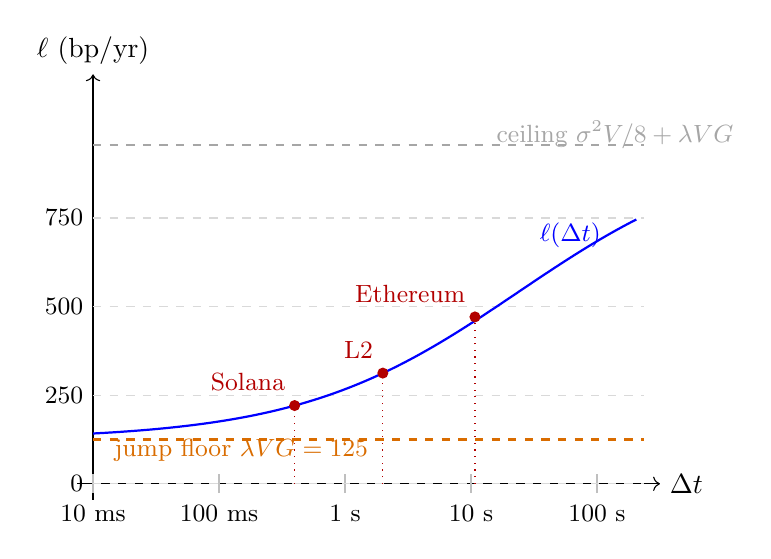
\begin{tikzpicture}[scale=1.0]
  % log-x axis from 0.01 s to 100 s, y = rate bp/yr 0..1000
  % x mapped: X = 1.6*(log10(dt)+2)  -> dt=0.01 -> 0 ; dt=100 -> 6.4
  % ell(dt) = 831.5*F + 125.2, F = 1/(1+sqrt2*kappa), kappa = 5e-4/(0.8156*sqrt(dt/3.15576e7))
  % kappa(dt) = 5e-4/(0.8156*sqrt(dt)/5618) = 3.446/sqrt(dt)   [dt in seconds]
  % => F = 1/(1+4.870/sqrt(dt))
  \def\YS{0.0045}   % y scale: bp -> cm
  \draw[->] (-0.2,0) -- (7.2,0) node[right] {$\dt$};
  \draw[->] (0,-0.2) -- (0,5.2) node[above] {$\ell$ (bp/yr)};
  % gridlines / ticks
  \foreach \i/\lab in {0/10 ms, 1.6/100 ms, 3.2/1 s, 4.8/10 s, 6.4/100 s}{
     \draw[gray!50] (\i,-0.12) -- (\i,0.12); \node[below, font=\small] at (\i,-0.15) {\lab};}
  \foreach \v in {0,250,500,750}{
     \draw[gray!30, dashed] (0,{\v*\YS}) -- (7,{\v*\YS});
     \node[left, font=\small] at (0,{\v*\YS}) {\v};}
  % ceiling
  \draw[gray!70, dashed] (0,{956*\YS}) -- (7,{956*\YS});
  \node[gray!70, right, font=\small] at (5.0,{985*\YS}) {ceiling $\sigma^2V/8 + \lambda VG$};
  % floor
  \draw[orange!85!black, thick, dashed] (0,{125.2*\YS}) -- (7,{125.2*\YS});
  \node[orange!85!black, right, font=\small] at (0.15,{95*\YS}) {jump floor $\lambda VG = 125$};
  % ell curve: X in [0,6.4], dt = 10^(X/1.6 - 2)
  \draw[thick, blue, domain=0:6.9, samples=140] plot
     (\x, {\YS*(125.2 + 831.5/(1 + 4.870/sqrt(pow(10,\x/1.6-2))))});
  \node[blue, right, font=\small] at (5.55,{700*\YS}) {$\ell(\dt)$};
  % deployed block times
  \foreach \dtv/\Xv/\lab in {0.4/2.56/Solana, 2/3.68/L2, 12/4.85/Ethereum}{
     \draw[red!70!black, dotted] (\Xv,0) -- (\Xv,{\YS*(125.2 + 831.5/(1 + 4.870/sqrt(\dtv)))});
     \fill[red!70!black] (\Xv,{\YS*(125.2 + 831.5/(1 + 4.870/sqrt(\dtv)))}) circle (2pt);}
  \node[red!70!black, font=\small, anchor=south east] at (2.56,{235*\YS}) {Solana};
  \node[red!70!black, font=\small, anchor=south east] at (3.68,{325*\YS}) {L2};
  \node[red!70!black, font=\small, anchor=south east] at (4.85,{485*\YS}) {Ethereum};
\end{tikzpicture}
\caption{The LVR rate against block time on a log scale, at the paper's calibration. The curve rises from the jump floor $\lambda VG = 125$ bp/yr toward the ceiling $\sigma^2V/8 + \lambda VG = 956$ bp/yr. The approach to the floor on the left is the $\sqrt{\dt}$ law of Corollary~\ref{cor:floor} --- visibly lazy, which is the point: at every deployed block time (red dots) the curve is still far above the floor. Note how much of the horizontal axis, several decades below Solana's $400$~ms, is needed before the floor actually binds.}
\label{fig:elldt}
\end{figure}

\subsection{The floor as un-recoverable LVR}

There is a sharper way to say what the floor is, using the fee-split accounting introduced in Section~\ref{sec:setup}. Since $\mathrm{ARB} + \mathrm{FEE} \approx \mathrm{LVR}$ and $\ell$ is the $\mathrm{ARB}$ half, the multiplier in each channel is precisely the \emph{share of that channel's frictionless LVR that leaks to arbitrageurs} rather than returning to LPs as fees:
\[
\text{diffusion channel: } \; F(\kappa) : 1 - F(\kappa),
\qquad
\text{jump channel: } \; \Psi(\gamma/\delta) : 1 - \Psi(\gamma/\delta).
\]
Shortening blocks drives $F \to 0$ and thus returns essentially all diffusion-LVR to LPs as fee income. On the jump channel the split is a function of $\gamma/\delta$ alone, with no $\dt$ in it, because a jump exceeding the band is cleared at the next block whatever the block rate is. At the calibration $\gamma/\delta = 0.0260$, so
\[
\Psi(0.0260) \;=\; 0.9595,
\]
and fees recover only $1 - \Psi(\gamma/\delta) = 4.1\%$ of jump-LVR. The other $96\%$ is the floor.

This is the paper's most actionable claim, and it follows from~\eqref{eq:Gclosed} alone: \textbf{the lever against the floor is $\gamma/\delta$ --- fee-tier design --- not the block schedule.}

\section{Theorem 4: the planner's block-time optimum}\label{sec:planner}

\subsection{The cost side}

Corollary~\ref{cor:floor} says shorter blocks always mean less LVR, which taken alone would recommend $\dt \to 0$. What stops that is the cost of producing blocks.

\paragraph{The physical cost.} Each block requires a fixed quantum of work regardless of how long the interval was: gossip and propagation~\cite{decker2013information}, BLS aggregation over committee attestations~\cite{buterin2022paths}, and view-change/commit overhead in committee-based consensus~\cite{benhaim2024scaling}. Croman et al.~\cite{croman2016scaling} identify per-block bandwidth as the binding scaling constraint. Holding per-block work fixed, halving the interval doubles the rate at which the work occurs, so the chain-level cost rate is
\[
R(\dt) \;=\; \frac{r}{\dt}.
\]

\paragraph{Assumption: issuance proxies the resource cost.} The true resource cost --- hardware, bandwidth, energy --- is not directly observable, so the paper calibrates $r$ from the chain's native-token issuance. This is a proxy and it is biased in both directions: issuance \emph{overstates} the resource cost where it acts as a growth subsidy, and \emph{understates} it where validators are additionally funded by fees and MEV~\cite{buterin2022paths,beccuti2025staking}. The bias shifts the level of $c$ and therefore moves $\dt^{\mathrm{opt}}$; Section~\ref{sec:calibration} reports the sensitivity, which is large --- nearly two orders of magnitude across the plausible range of $c$. This is the weakest link in the numerical conclusion and the paper says so.

\paragraph{Assumption: pro-rata attribution by value secured.} A pool with TVL $V$ on a chain of native-token market capitalization $V_{\mathrm{chain}}$ inherits
\[
c(\dt) \;=\; R(\dt)\cdot\frac{V}{V_{\mathrm{chain}}} \;=\; \frac{c}{\dt},
\qquad c \;:=\; r\cdot\frac{V}{V_{\mathrm{chain}}} .
\]
A finer attribution would also charge the LP for ETH-side dilution through issuance; the paper abstracts from that channel. Note for later that $c \propto V$ --- this is what makes the optimum independent of pool size.

The planner minimizes
\begin{equation}\label{eq:W}
W(\dt) \;=\; \ell(\dt) \;+\; \frac{c}{\dt}.
\end{equation}

\paragraph{Assumption: the objective is LP-LVR-only.} $W$ omits MEV redistribution, finality, censorship resistance, and oracle freshness, all of which are genuinely affected by $\dt$. So $\dt^{\mathrm{opt}}$ is an LP-side \emph{input} to a social-welfare problem, not a prescription. The omission is also one-signed in a useful way: several of the omitted terms (finality, propagation safety) push toward longer blocks, so a fuller treatment would move $\dt^{\mathrm{opt}}$ up rather than down.

\subsection{From the FOC to a cubic}

Only the diffusion term depends on $\dt$. \emph{This one observation drives every result in the theorem}: once $\ell'$ contains no jump parameters, neither does the first-order condition.

Differentiate. With $\kappa = \gamma\sigma^{-1}\dt^{-1/2}$ we have $d\kappa/d\dt = -\kappa/(2\dt)$, so using~\eqref{eq:Fprime},
\begin{equation}\label{eq:ellprime}
\ell'(\dt) \;=\; \frac{\sigma^2V}{8}\,F'(\kappa)\cdot\Big(-\frac{\kappa}{2\dt}\Big)
\;=\; \frac{\sigma^2V}{8}\cdot\frac{\sqrt2\,\kappa}{2\dt\,(1+\sqrt2\kappa)^2}
\;=\; \frac{\sigma^2V}{8}\cdot\frac{\eta}{2\dt\,(1+\eta)^2} \;>\; 0 .
\end{equation}
The first-order condition $W'(\dt) = 0$ is $\ell'(\dt) = c/\dt^2$. Multiply through by $\dt^2$:
\[
\dt^2\,\ell'(\dt) \;=\; \frac{\sigma^2 V\dt}{16}\cdot\frac{\eta}{(1+\eta)^2} \;=\; c .
\]
Now eliminate $\dt$ in favour of $\eta$. From $\eta = \sqrt2\gamma/(\sigma\sqrt{\dt})$ we get $\sigma^2\dt = 2\gamma^2/\eta^2$, so
\[
\frac{V}{16}\cdot\frac{2\gamma^2}{\eta^2}\cdot\frac{\eta}{(1+\eta)^2}
\;=\; \frac{V\gamma^2}{8\,\eta\,(1+\eta)^2} \;=\; c,
\]
which rearranges to

\begin{theorem}[Optimal block time; paper Thm.~3]\label{thm:planner}
\begin{equation}\label{eq:cubic}
\boxed{\;\eta^{\mathrm{opt}}\big(1+\eta^{\mathrm{opt}}\big)^2 \;=\; \frac{V\gamma^2}{8c},
\qquad
\dt^{\mathrm{opt}} \;=\; \frac{2\gamma^2}{\sigma^2\,(\eta^{\mathrm{opt}})^2}. \;}
\end{equation}
\end{theorem}

\subsection{Uniqueness, and why it is a minimum}

Write $q(\dt) := \dt^2\ell'(\dt) = V\gamma^2/\big(8\eta(1+\eta)^2\big)$, so that $\dt^2W'(\dt) = q(\dt) - c$. The map $\eta \mapsto \eta(1+\eta)^2$ is a strictly increasing bijection of $(0,\infty)$ onto itself (each factor is positive and increasing), so $q$ is strictly decreasing in $\eta$ and hence strictly \emph{increasing} in $\dt$, with $q \to 0$ as $\dt\to0$ and $q\to\infty$ as $\dt\to\infty$.

Therefore $W'$ changes sign exactly once, from negative to positive, and $W$ has a unique interior global minimum, located where $q = c$. Existence and uniqueness for every $c > 0$ come free from the bijection. $\qquad\blacksquare$

\subsection{Cardano's closed form}

Equation~\eqref{eq:cubic} is $\eta^3 + 2\eta^2 + \eta - A = 0$ with $A := V\gamma^2/(8c)$. Depress it by $\eta = w - \tfrac23$:
\begin{align*}
(w-\tfrac23)^3 &= w^3 - 2w^2 + \tfrac43 w - \tfrac{8}{27},\\
2(w-\tfrac23)^2 &= 2w^2 - \tfrac83 w + \tfrac89,\\
(w-\tfrac23) &= w - \tfrac23 .
\end{align*}
The $w^2$ terms cancel and the rest collects to
\[
w^3 - \tfrac13 w - \big(\tfrac{2}{27} + A\big) \;=\; 0 .
\]
This is $w^3 + pw + q = 0$ with $p = -\tfrac13$ and $q = -(\tfrac2{27}+A)$. Cardano's substitution $w = u^{1/3} + u'^{1/3}$ requires
\[
u + u' \;=\; -q \;=\; \tfrac{2}{27} + A,
\qquad
u\,u' \;=\; -\frac{p^3}{27} \;=\; \frac{1}{729},
\]
so $u$ and $u'$ are the roots of $t^2 - (\tfrac2{27}+A)t + \tfrac1{729} = 0$. With $B := A/2 + 1/27$ the larger root is $u = B + \sqrt{B^2 - 1/729}$, and since $u' = 1/(729u)$ we have $u'^{1/3} = \tfrac19 u^{-1/3}$. Hence
\begin{equation}\label{eq:cardano}
\boxed{\;\eta^{\mathrm{opt}} \;=\; u^{1/3} + \tfrac19 u^{-1/3} - \tfrac23,
\qquad u = B + \sqrt{B^2 - \tfrac1{729}}, \quad B = \tfrac{A}{2} + \tfrac1{27}. \;}
\end{equation}
The discriminant $B^2 - 1/729$ is positive for every $A > 0$, so there is exactly one real root, matching the uniqueness argument above. Writing the smaller cube root as $\tfrac19u^{-1/3}$ rather than computing $u'$ directly avoids catastrophic cancellation when $A$ is small.

\paragraph{Worked check.} At the calibration, $A = V\gamma^2/(8c) = 10^6(5\times10^{-4})^2/(8\times2.6\times10^{-3}) = 12.019$. Then $B = 6.047$, $u = 6.047 + \sqrt{36.56 - 0.00137} = 12.093$, $u^{1/3} = 2.2965$, and
\[
\eta^{\mathrm{opt}} = 2.2965 + \tfrac19(2.2965)^{-1} - \tfrac23 = 1.6771,
\qquad
\dt^{\mathrm{opt}} = \frac{2\gamma^2}{\sigma^2(\eta^{\mathrm{opt}})^2} = 8.44\ \text{s}.
\]
This reproduces \texttt{code.py}'s \texttt{v\_opt} and \texttt{dt\_opt\_sec} exactly.

\subsection{Comparative statics}

Differentiating~\eqref{eq:cubic} gives four sensitivities. The first two are unsurprising; the last two are the paper's point.

\paragraph{$\partial\dt^{\mathrm{opt}}/\partial c > 0$.} More expensive consensus lengthens the optimum: the planner amortizes the per-block cost over longer intervals and accepts more LVR per block. The dependence is strong:
\[
c\times10^{5} = (500,\ 260,\ 90,\ 30,\ 2)
\quad\Longrightarrow\quad
\dt^{\mathrm{opt}} = (15.4,\ 8.4,\ 3.4,\ 1.4,\ 0.20)\ \text{s}.
\]

\paragraph{$\partial\dt^{\mathrm{opt}}/\partial\gamma$ is U-shaped.} At very low $\gamma$ the multiplier $F$ sits near $1$ and shortening blocks barely suppresses diffusion-LVR; at very high $\gamma$ the multiplier is already crushed and shortening buys nothing more. The interior minimum sits where the block schedule is actually an effective lever.

\paragraph{$\partial\dt^{\mathrm{opt}}/\partial\lambda = \partial\dt^{\mathrm{opt}}/\partial m = \partial\dt^{\mathrm{opt}}/\partial\delta = 0$.}
No jump parameter appears in~\eqref{eq:cubic}. Jumps shift the \emph{level} of $W$ by the constant $\lambda VG$ and leave the \emph{slope} untouched, and the FOC sees only the slope.

This deserves a moment, because the naive intuition is the opposite. One might expect a planner facing a jumpier market to shorten blocks defensively. Theorem~\ref{thm:planner} says no: a planner who knows jumps are frequent and large should choose exactly the same block time as one who knows they are rare and small. Block time is not a lever against jumps at all --- pulling it in either direction leaves the jump contribution unchanged --- so it is not surprising, on reflection, that the optimal amount of pulling is unaffected. \emph{Jumps change what is achievable, not what should be chosen.}

\paragraph{$\partial\dt^{\mathrm{opt}}/\partial V = 0$.} Because $c = rV/V_{\mathrm{chain}}$ is proportional to $V$, the right-hand side of~\eqref{eq:cubic} is $V\gamma^2/(8c) = \gamma^2 V_{\mathrm{chain}}/(8r)$, in which $V$ has cancelled. The optimum is a property of the chain and the fee tier, not of the pool. A \$100k pool and a \$10M pool want the same block time.

\paragraph{Caveat: exactness of the invariance.} The $\lambda$-invariance is exact for the closed form~\eqref{eq:main}, but~\eqref{eq:main} carries the remainder $\mathcal E(\dt)$ of Proposition~\ref{prop:err}, whose interaction and block-clock terms \emph{do} depend on $\lambda$ and on $\dt$. So the invariance is a leading-order property, not a structural symmetry. Quantitatively the correction is negligible: the whole remainder is under $0.07\%$ of the rate, and its $\dt$-derivative is smaller still.
\section{Where the numbers come from}\label{sec:calibration}

The paper's Section~7 states the calibration in two sentences. Since every headline number depends on it, this section spells out the estimators. The price parameters are estimated from \textbf{Binance ETH/USDT $5$-minute closes, January 2020 -- June 2026}: $2{,}373$ usable days, $6.50$ years.

\paragraph{Assumption: a centralized-exchange price is the right reference.} The LVR construct needs an external price against which the pool is arbitraged. Binance ETH/USDT is the deepest venue for the pair, so its mid is the best available proxy for the price an arbitrageur actually trades against. Using $5$-minute closes rather than tick data is a deliberate compromise: coarse enough to suppress microstructure noise, which would inflate realized variance at tick frequency, and fine enough that $288$ observations per day support the jump test below. Bars separated by anything other than exactly $300{,}000$~ms are dropped, so exchange outages do not manufacture spurious jumps.

\subsection{\texorpdfstring{$\sigma$}{sigma} from bipower variation}

Let $x_{d,i}$ be the $i$-th $5$-minute log return on day $d$, with $n$ returns that day. The obvious daily statistic, realized variance $\mathrm{RV}_d = \sum_i x_{d,i}^2$, converges as the sampling interval shrinks to the \emph{total} quadratic variation --- continuous \emph{plus} jumps. Since $\sigma$ in the model is the coefficient of the Brownian part only, $\mathrm{RV}$ is the wrong estimator, and we need the continuous part in isolation.

\emph{Bipower variation} (Barndorff-Nielsen and Shephard~\cite{bns2004power}) supplies it:
\begin{equation}\label{eq:bpv}
\mathrm{BV}_d \;=\; \frac{1}{\mu_1^2}\cdot\frac{n}{n-1}\sum_{i=2}^{n}|x_{d,i}|\,|x_{d,i-1}|,
\qquad \mu_1 := \E|Z| = \sqrt{2/\pi}.
\end{equation}
The mechanism is worth understanding, because it is what makes the continuous/jump split possible at all. A jump inflates \emph{one} return. Bipower variation multiplies \emph{adjacent} returns, so a single large return is always paired with a neighbour that is merely diffusive, and the product stays $O(\sqrt{\Delta})$ instead of $O(1)$. As the sampling interval shrinks the probability of two adjacent jumps vanishes, so $\mathrm{BV}$ converges to the continuous quadratic variation alone. The factor $\mu_1^{-2} = \pi/2$ corrects for $\E\big[|Z_1||Z_2|\big] = \mu_1^2$ under normality, so that $\mathrm{BV}$ is unbiased for $\int\sigma^2$ in the absence of jumps.

Averaging over days and annualizing with $365.25$,
\[
\hat\sigma \;=\; \sqrt{365.25\cdot\overline{\mathrm{BV}}} \;=\; \mathbf{0.8156} \quad \text{per } \sqrt{\text{yr}}.
\]

\subsection{\texorpdfstring{$\lambda$}{lambda} from the Lee--Mykland test}

Bipower variation gives the continuous part but says nothing about $\lambda$ and $\delta$ separately. Obtaining them requires identifying \emph{which} returns are jumps. Lee and Mykland~\cite{leemykland2008jumps} give the standard test: standardize each return by a \emph{local} volatility estimate built from its neighbours, and flag returns too large to be diffusive.

\paragraph{The statistic.} With a window of $K = 288$ bars (one day), estimate the local variance just before bar $i$ by a trailing bipower average and standardize:
\begin{equation}\label{eq:lm}
\hat s_i^2 \;=\; \frac{1}{K-2}\sum_{j=i-K+2}^{i-1} |x_j|\,|x_{j-1}|,
\qquad
\mathcal L_i \;=\; \frac{x_i}{\hat s_i}.
\end{equation}
Using bipower rather than squared returns for $\hat s_i$ matters here too: it keeps a jump inside the window from inflating the yardstick against which its neighbours are tested.

\paragraph{The critical value.} Under the null of no jumps, $\mathcal L_i$ is approximately normal scaled by $\mu_1$, and the \emph{maximum} of $n$ such statistics has a Gumbel limit:
\[
\frac{\max_i|\mathcal L_i| - C_n}{S_n} \;\xrightarrow{d}\; \text{Gumbel},
\quad
C_n = \frac{(2\log n)^{1/2}}{\mu_1} - \frac{\log\pi + \log\log n}{2\mu_1 (2\log n)^{1/2}},
\quad
S_n = \frac{1}{\mu_1 (2\log n)^{1/2}}.
\]
At level $\alpha$ the threshold is $C_n + S_n\cdot\big(-\log(-\log(1-\alpha))\big)$, and bar $i$ is flagged when $|\mathcal L_i|$ exceeds it. Because the limit law is that of the maximum, this controls the error rate over the \emph{whole sample} rather than per observation, which is why $\alpha = 1\%$ is a stringent level here rather than a lax one.

\paragraph{Result.} With $n = 682{,}659$ testable bars the threshold is $|\mathcal L_i| > 7.16$, and $1{,}808$ bars clear it --- a detection rate of $0.265\%$. Over the $6.50$-year sample,
\[
\hat\lambda \;=\; \frac{1808}{6.50} \;=\; \mathbf{283.3}\ \text{/yr}.
\]

\subsection{\texorpdfstring{$\delta$}{delta} from the detected jumps, bias-corrected}

A flagged return is not a pure jump. It is a jump \emph{plus} that bar's diffusive move,
\[
x_i \;=\; J_i + \sigma\sqrt{\Delta}\,Z_i \quad\text{on a flagged bar},
\qquad \Delta = \frac{5\ \text{min}}{1\ \text{yr}},
\]
so taking $\hat\delta^2 = \overline{x_i^2}$ over flagged bars would count the diffusion twice --- once in $\hat\sigma$ and again in $\hat\delta$. Subtracting the diffusive variance of a single bar,
\begin{equation}\label{eq:deltahat}
\hat\delta^2 \;=\; \max\Big(\overline{x_i^2} \;-\; \hat\sigma_{\mathrm{trunc}}^2\,\Delta,\; 0\Big)
\qquad\Longrightarrow\qquad
\hat\delta \;=\; \mathbf{0.0192},
\end{equation}
where $\hat\sigma_{\mathrm{trunc}}$ is realized volatility over the \emph{non}-flagged bars. This is what the paper means by ``correcting the detected jump sizes for their diffusive component.''

\paragraph{The three parameters together.} Collecting,
\[
\hat\sigma = 0.8156, \qquad \hat\lambda = 283.3\ \text{/yr}, \qquad \hat\delta = 0.0192,
\]
from which $\gamma/\delta = 0.0260$, $\Psi(\gamma/\delta) = 0.9595$, $G = 4.51\times10^{-5}$, and hence the diffusion ceiling $\sigma^2V/8 = 832$~bp/yr and the jump floor $\lambda VG = 125$~bp/yr that anchor the paper's Section~7. Note that the floor depends on $\lambda$ and $\delta$ almost entirely through the product $\lambda\delta^2$ --- the jump variance rate --- since $\Psi(\gamma/\delta)$ is within $4\%$ of $1$; the split between ``many small jumps'' and ``few large ones'' matters only through that factor.

\paragraph{Assumption: the estimation is external to \texttt{code.py}.} The routines in \texttt{code.py} take $(\sigma,\lambda,\delta)$ as fixed inputs at the top of the file and reproduce every number in the paper from them. The estimation above is a separate step run once against the exchange data; the numerical experiments of Section~\ref{sec:experiments} test the \emph{model}, not the calibration.

\subsection{The consensus cost}

The remaining parameter, $c$, is not estimated from market data but constructed:
\begin{itemize}[leftmargin=2em]
\item Ethereum's gross consensus issuance is $\approx\$1.7$B/yr against $V_{\mathrm{chain}} \approx \$208$B.
\item Staking sits near $30\%$ of supply against Drake's security-optimal $\approx1/4$~\cite{drake2025croissant,elowsson2024endgame}, so issuance overpays by $30/25 = 1.2$; scaling by $0.83$ gives $\approx\$1.4$B/yr as a minimum-viable proxy for the resource cost.
\item Pro-rata by value secured, $V/V_{\mathrm{chain}} = 4.8\times10^{-6}$, gives $\approx\$6{,}750$/yr per \$1M of TVL; dividing by $\approx2.6\times10^6$ blocks/yr,
\[
c \;\approx\; 260\times10^{-5}\ \text{USD/block per \$1M TVL}.
\]
\end{itemize}
Every step here is a modelling choice rather than a measurement, which is why the paper reports $\dt^{\mathrm{opt}}$ across $c \in (2,\dots,500)\times10^{-5}$, a range over which the optimum moves from $0.20$~s to $15.4$~s. The cost calibration, not the price calibration, is what the block-time conclusion is most sensitive to.

\paragraph{The remaining parameters are choices, not estimates.} $m = 0$ (symmetric jumps, required for the closed form~\eqref{eq:Gclosed}), $\gamma = 5$~bp (the Uniswap $0.05\%$ tier), and $V = \$1$M (a representative pool --- and by Theorem~\ref{thm:planner} the optimum does not depend on it).

\section{The numerical experiments}\label{sec:experiments}

Several claims in the paper are supported by computation rather than proof. This section says what each experiment computes, what it is a check on, and what it returns. All of them live in \texttt{code.py} and run with \texttt{python3 code.py}; the headline numbers need only the standard library, while the last two experiments additionally use \texttt{numpy}/\texttt{scipy}.

\subsection{Experiment 1: is the per-trade loss formula right?}

\paragraph{What it checks.} Everything downstream rests on the claim that a log-displacement $\xi$ costs the LP $\tfrac{V}{2}(e^{\xi/2}-1)^2$, truncated to $\tfrac{V}{8}\xi^2$. That claim is an algebraic identity, but it is worth confirming against the arbitrage profit computed the long way --- from reserves --- as in Milionis et al.~\cite[Lemma~2]{milionis2023automated}.

\paragraph{How.} The routine \texttt{arb\_per\_trade} evaluates three expressions for the same trade, with the pool at $Se^{-z}$ before and $Se^{-\gamma}$ after:
\begin{enumerate}[leftmargin=2em]
\item their Lemma~2 verbatim, $S\big(x(Se^{-z}) - x(Se^{-\gamma})\big) + e^{\gamma}\big(y(Se^{-z}) - y(Se^{-\gamma})\big)$;
\item the CPMM closed form $\sqrt{LS}\,e^{\gamma/2}\cdot 4\sinh^2\!\big(\tfrac{z-\gamma}{4}\big)$;
\item the quadratic truncation $\tfrac{V}{8}(z-\gamma)^2$.
\end{enumerate}

\paragraph{Result.} (1) and (2) agree to every digit printed, confirming the closed form. (3) departs from them by $2.5\times10^{-4}$ relative at $z = 0.01$ and $3.0\times10^{-4}$ at $z = 0.05$ --- the curvature truncation of Proposition~\ref{prop:err}(c), here visible directly rather than through a bound.

\subsection{Experiment 2: does \texorpdfstring{$\mathrm{ARB} + \mathrm{FEE} = \mathrm{LVR}$}{ARB + FEE = LVR} actually hold?}

\paragraph{What it checks.} The interpretation of $\ell$ as the arbitrage half of a split (Section~\ref{sec:setup}) is doing real work in the paper's conclusions --- particularly the claim that fees recover only $4.1\%$ of jump-LVR. If the identity were assumed and $\mathrm{FEE}$ defined as a residual, the claim would be circular.

\paragraph{How.} \texttt{fee\_bp} computes fee income \emph{directly}, never as a residual: fee rate $\gamma$ times trade size, with trade size $= \tfrac{V}{4}|\xi|$ at leading order, integrated over the stationary law for the diffusion channel and over the jump law for the jump channel. It is then compared with the frictionless LVR of Theorem~\ref{thm:1}, computed independently.

\paragraph{Result.} At every block time tested, $\mathrm{ARB} + \mathrm{FEE} = 961.18$~bp/yr against a frictionless LVR of $961.29$~bp/yr --- agreement to $0.011\%$, the residual being exactly the quadratic truncation. Note that the split moves enormously with $\dt$ (from $471{:}491$ at $12$~s to $162{:}799$ at $50$~ms) while the total does not move at all. That invariance of the total is the content of Theorem~\ref{thm:1}, and seeing it survive the fee machinery is a strong check on the whole construction.

\subsection{Experiment 3: how large is the remainder \texorpdfstring{$\mathcal E$}{E}, really?}\label{sec:expquad}

\paragraph{What it checks.} Proposition~\ref{prop:err} gives an upper bound on $\mathcal E$. A bound is only useful if it is not wildly loose, so this experiment computes the \emph{realized} remainder by evaluating the exact rate~\eqref{eq:ratestat} without the approximations.

\paragraph{How.} \texttt{exact\_lvr\_bp} performs a deterministic quadrature. Conditional on $N = n$ jumps in an interblock interval, the elapsed time is $\mathrm{Gamma}(n+1, \beta+\lambda)$ and the increment is $\mathcal N(nm,\ \sigma^2T + n\delta^2)$; the resulting mixture is integrated against the \emph{post-block} law (atoms at $\pm\gamma$ plus the uniform band), summing over $n$ up to $3$. For $n = 0$ the time-mixture is exactly Laplace, so that term is done in closed form rather than numerically. Both the first-order loss $\tfrac{V}{8}\xi^2$ and the full concavity loss $\tfrac{V}{2}(e^{\xi/2}-1)^2$ are computed, which separates the $O(\lambda\dt)$ errors from the curvature error. It is ``quasi''-exact only in that the post-block law still ignores jump feedback into the stationary distribution, an $O(\lambda\dt) = O(10^{-5})$ effect.

\paragraph{Result.}
\begin{center}
\begin{tabular}{lrrrrr}
\toprule
$\dt$ & closed form & quasi-exact & $\mathcal E_{O(\lambda\dt)}$ & $\mathcal E_{\mathrm{curv}}$ & Prop.~\ref{prop:err} bound \\
\midrule
$12$ s   & $470.55$ & $470.71$ & $+0.143$ & $+0.021$ & $0.341$ \\
$2$ s    & $312.29$ & $312.37$ & $+0.062$ & $+0.020$ & $0.100$ \\
$400$ ms & $220.89$ & $220.95$ & $+0.040$ & $+0.020$ & $0.063$ \\
$50$ ms  & $161.93$ & $161.98$ & $+0.032$ & $+0.020$ & $0.053$ \\
\bottomrule
\end{tabular}
\end{center}
Three things to read off. The realized remainder never exceeds $0.035\%$ of the rate. The bound is loose by a factor of $2$ at $12$~s but \emph{tight} in the fast-block limit, which is where it matters, since that is where the floor claim lives. And the remainder is positive everywhere, as Proposition~\ref{prop:err} predicts from convexity --- so the closed form understates, and $\lambda VG$ is a genuine lower bound on the limiting rate.

\paragraph{A caution learned the hard way.} An earlier version of this quadrature used a midpoint rule on the Gamma time-mixture with $60$ nodes, whose weights summed to $1.038$ rather than $1$. The resulting $4\%$ over-weighting appeared as a spurious $+5$~bp/yr ``interaction remainder'' --- roughly $100\times$ the true value --- and was briefly mistaken for a real effect. The routine now normalizes the weights explicitly and warns if the truncated Gamma tail drops more than $10^{-5}$ of mass. When a numerical experiment reports an anomaly two orders of magnitude above the analytical bound, suspect the quadrature before the theory.

\subsection{Experiment 4: how bad is the reset-to-zero shortcut?}

\paragraph{What it checks.} The correction at the heart of Section~\ref{sec:resettrap}. Since both $F$ and $\Psi$ are available in closed form this is a two-line evaluation rather than a simulation, but it is reported in \texttt{code.py} because the magnitude is easy to underestimate.

\paragraph{Result.} $F/\Psi = 2.73$ at $12$~s, $76$ at $2$~s, $3.9\times10^{7}$ at $400$~ms. See the table in Section~\ref{sec:resettrap}.

\subsection{Experiment 5: the deterministic-slot constant}\label{sec:schedule}

\paragraph{What it checks.} The Poisson-arrival assumption. Real chains produce blocks on a schedule, and the paper claims the same functional shape survives with a different constant. That claim is established numerically, not analytically, and this is the experiment behind it.

\paragraph{How.} Under a deterministic schedule there is no PASTA property and no closed-form stationary law, so \texttt{F\_determ} finds the post-block law by \textbf{iterating it to its fixed point}. The state is a measure on $[-\gamma,\gamma]$ consisting of two atoms at $\pm\gamma$ (where clipped mass lands) plus a density on the interior. One iteration applies the transition: convolve with $\mathcal N(0,\sigma^2\dt)$, keep the mass that lands inside the band as density, and collapse the mass beyond each edge onto the corresponding atom. Iterate to a tolerance of $10^{-14}$ on the total-variation change. Then evaluate $\ell_{\mathrm{diff}} = \E[(|M+X|-\gamma)_+^2]/(8\dt)$ against the converged law, and divide by $\sigma^2/8$ to read off $F_{\det}$.

\paragraph{Result.} The Poisson formula keeps its shape,
\[
F(\kappa) \;\approx\; \frac{C}{C+\kappa},
\]
with $C = 1/\sqrt2 = 0.7071$ \emph{exactly} for Poisson blocks and $C = 0.5826$ for deterministic slots, the fit being accurate to $0.083\%$ or better across three decades of $\dt$:
\begin{center}
\begin{tabular}{lrrrrr}
\toprule
$\dt$ & $\kappa$ & $F_{\text{Poisson}}$ & $F_{\det}$ (iterated) & $C_{\det}/(C_{\det}+\kappa)$ & inflation \\
\midrule
$60$ s   & $0.4449$  & $0.6138$ & $0.5675$ & $0.5670$ & $8.2\%$ \\
$12$ s   & $0.9948$  & $0.4155$ & $0.3693$ & $0.3693$ & $12.5\%$ \\
$2$ s    & $2.4367$  & $0.2249$ & $0.1930$ & $0.1930$ & $16.6\%$ \\
$400$ ms & $5.4486$  & $0.1149$ & $0.0966$ & $0.0966$ & $18.9\%$ \\
$50$ ms  & $15.4108$ & $0.0439$ & $0.0364$ & $0.0364$ & $20.4\%$ \\
\bottomrule
\end{tabular}
\end{center}

\paragraph{Identifying the constant.} The value $0.5826$ is not arbitrary: to six digits it is
\[
C_{\det} \;=\; -\frac{\zeta(1/2)}{\sqrt{2\pi}} \;=\; 0.5825971\ldots,
\]
the continuity-correction constant of Broadie, Glasserman and Kou~\cite{broadie1997continuity} for discretely-monitored barrier options. That is exactly the right constant to expect. Discrete monitoring lets the walk \emph{overshoot} the barrier between observations, and the standard remedy is to shift the barrier outward by $C_{\det}$ times the per-step standard deviation. Here the ``barrier'' is the band edge $\pm\gamma$ and the per-step standard deviation is $\sigma\sqrt{\dt}$, so the effective band is $\gamma + C_{\det}\sigma\sqrt{\dt}$ --- which is precisely what turns $1/(1+\kappa/C)$ into a formula with $C = C_{\det}$.

\paragraph{Consequences.} Randomizing the slot inflates the diffusion channel by $12.5\%$ at $12$~s and by $C_{\text{Poisson}}/C_{\det} - 1 = 21.4\%$ in the fast-block limit. So the Poisson assumption is \emph{conservative}: it overstates arbitrage profit relative to a real deterministic chain, consistent with Nezlobin and Tassy's~\cite{nezlobin2025lvr} theorem that the deterministic schedule minimizes arbitrage profit among distributions with a given mean. Since the planner's cubic~\eqref{eq:cubic} carries $C$ through as $v(1+v)^2 = V\gamma^2/(16cC^2)$ with $v = \kappa/C$, the optimum moves from $8.44$~s to $8.87$~s, a shift of $5.1\%$ --- small enough that the paper's conclusion is unaffected by the assumption it is most often questioned on.

\subsection{Experiment 6: root-finding for the regime boundary}

Two scalar equations are solved numerically rather than in closed form. Both are strictly monotone, so bisection is used and convergence is guaranteed.
\begin{itemize}[leftmargin=2em]
\item \emph{The crossover $\dt_\times$}, where the two channels are equal: $F(\kappa) = 8\lambda G/\sigma^2 = 0.1511$, giving $\kappa_\times = 3.97$ and $\dt_\times = 0.75$~s. Here $F$ is invertible in closed form, so this is direct.
\item \emph{The $50\%$ diffusion-share volatility} at $\dt = 12$~s, solving $(\sigma^2/8)F(\kappa(\sigma)) = \lambda G$ for $\sigma$: bisection on $[0.05, 3.0]$ for $200$ iterations gives $\sigma = 0.5549$. Below this the pool is jump-dominated at Ethereum's slot; the calibrated $\sigma = 0.8156$ sits well above it, which is why the baseline reads $73\%$ diffusion.
\end{itemize}

\subsection{What is \emph{not} verified numerically}

For honesty about the evidential status of each claim: Theorems~\ref{thm:1}, \ref{thm:2} and~\ref{thm:planner}, Lemmas~\ref{lem:pi} and~\ref{lem:G}, Corollary~\ref{cor:floor} and the bound in Proposition~\ref{prop:err} are proved. The \emph{tightness} of that bound (Experiment~3), the deterministic-slot constant and the accuracy of the $C/(C+\kappa)$ fit (Experiment~5) are numerical findings, established at the calibrated parameters and a handful of block times, not proved in general. The identification of $0.5826$ with $-\zeta(1/2)/\sqrt{2\pi}$ is a numerical match to six digits plus a structural argument, not a derivation.

\section{Summary of the logical flow}

\begin{enumerate}[leftmargin=2em]
\item \textbf{Setup.} Price $=$ Merton jump-diffusion. Pool $=$ constant product, $V = 2\sqrt{LP}$, $V'' = -x(P)/(2P) < 0$. LVR $=$ gap between the rebalancing strategy and the bonding curve. With fees, LVR \emph{splits} into $\mathrm{ARB} + \mathrm{FEE}$, and $\ell$ is the $\mathrm{ARB}$ half.

\item \textbf{Theorem~\ref{thm:1} (zero-fee LVR).} It\^o--L\'evy~\cite[Prop.~8.14]{cont2003financial} applied to $V(S_t)$, substituted into the LVR definition. The diffusion piece evaluates to $\sigma^2V/8$; the jump piece, via the algebraic identity $V(Pr) - V(P) - V'(P)P(r-1) = -\tfrac{V}{2}(\sqrt r - 1)^2$ and the marked-Poisson compensator~\cite[Prop.~8.8]{cont2003financial}, to $\tfrac{\lambda V}{2}\E[(e^{J/2}-1)^2]$. Neither term contains $\dt$ or $\gamma$.

\item \textbf{Lemma~\ref{lem:pi} (the stationary law).} With $\gamma > 0$ the mispricing $z$ is a \emph{persistent state} driven by two point processes: jumps pushing out, blocks pushing in. Its stationary law is uniform on the band with exponential tails, and $\Prob_\pi(|z|>\gamma) = 1/(1+\eta)$.

\item \textbf{The fee multiplier (paper Lemma~2).} $\ell_{\mathrm{diff}} = (\sigma^2V/8)F(\kappa)$ with $F(\kappa) = 1/(1+\sqrt2\kappa)$, which \emph{is} the stationary trade probability. The tail is algebraic, not Gaussian. Assuming instead that the pool re-pegs each block gives $\Psi(\kappa)$ and understates the channel by up to $4\times10^7$.

\item \textbf{Lemma~\ref{lem:G} (the jump coefficient).} $\ell_{\mathrm{jump}} = \lambda VG$ with $G = \tfrac18\E[(|J|-\gamma)^2\1\{|J|>\gamma\}] = (\delta^2/8)\Psi(\gamma/\delta)$ for $m=0$. The fee is measured against $\delta$, so no $\dt$ appears.

\item \textbf{Theorem~\ref{thm:2} and Proposition~\ref{prop:err}.} $\ell(\dt) = (\sigma^2V/8)F(\kappa) + \lambda VG + \mathcal E$, with $\mathcal E$ bounded by an interaction term, a block-clock term and a curvature term, together under $0.07\%$ of the rate.

\item \textbf{Corollary~\ref{cor:floor} (the floor).} $\ell \to \lambda VG > 0$ as $\dt \to 0$, approached only as $\sqrt{\dt}$: halving the block time removes $29.3\%$ of the diffusion term, forever. The floor is real but distant.

\item \textbf{Theorem~\ref{thm:planner} (the planner).} Minimizing $W = \ell + c/\dt$ gives the cubic $\eta(1+\eta)^2 = V\gamma^2/(8c)$, solvable by Cardano, with $\dt^{\mathrm{opt}} = 2\gamma^2/(\sigma^2\eta^2)$. Because the jump term is flat in $\dt$, it shifts the level of $W$ but not its slope: $\dt^{\mathrm{opt}}$ is invariant in $(\lambda, m, \delta)$ and, since $c \propto V$, in pool size too.
\end{enumerate}

\noindent In one sentence: \emph{jumps change what block-time policy can achieve, not what it should choose.}

\section*{Notation summary}

\begin{center}
\begin{tabular}{ll}
\toprule
Symbol & Meaning \\
\midrule
$S_t$, $P_t$ & external reference price; AMM pool marginal price \\
$z_t = \log(S_t/P_t)$ & log mispricing --- a \emph{persistent} state, never reset to $0$ \\
$\mu$, $\sigma$ & price drift, continuous volatility \\
$N_t$, $\lambda$ & jump counting process and its intensity \\
$J$, $m$, $\delta$ & log-jump size, its mean and standard deviation \\
$L$; $x(P), y(P)$ & constant-product invariant $xy = L$; reserves at price $P$ \\
$V(P) = 2\sqrt{LP}$ & pool value in numeraire \\
$\gamma$ & swap fee, in log-price units \\
$\dt$ & \emph{mean} block time (blocks are Poisson at rate $\beta = 1/\dt$) \\
$\pi$, $p(x)$ & stationary law of $z$ and its density~\eqref{eq:pi0} \\
$\theta = \sqrt{2/\dt}/\sigma$ & exponential tail rate of $\pi$; $1/\theta$ is one block's diffusive scale \\
$\kappa = \gamma/(\sigma\sqrt{\dt})$ & fee in units of the per-block diffusive move \\
$\eta = \sqrt2\,\kappa = \theta\gamma$ & the same, in the units natural to $\pi$ \\
$F(\kappa) = 1/(1+\sqrt2\kappa)$ & diffusion fee multiplier $=\Prob_\pi(|z|>\gamma)$ \\
$\Psi(x) = \E[(|Z|-x)_+^2]$ & truncated-normal second moment,~\eqref{eq:psi} \\
$G(\gamma;m,\delta^2)$ & jump-LVR coefficient,~\eqref{eq:G}; $=(\delta^2/8)\Psi(\gamma/\delta)$ at $m=0$ \\
$\mathcal E(\dt)$ & remainder in~\eqref{eq:main}, bounded in Prop.~\ref{prop:err} \\
$\ell(\dt)$ & LVR rate $=$ the $\mathrm{ARB}$ half of the fee split \\
$\dt_\times$ & block time at which the two channels are equal \\
$c$, $W(\dt)$ & per-block consensus cost per pool; planner objective $\ell + c/\dt$ \\
$\dt^{\mathrm{opt}}$ & planner's optimum, from the cubic~\eqref{eq:cubic} \\
$C$ & block-schedule constant: $1/\sqrt2$ Poisson, $-\zeta(1/2)/\sqrt{2\pi}$ deterministic \\
$\Phi$, $\varphi$ & standard normal CDF and density \\
\bottomrule
\end{tabular}
\end{center}

\begin{thebibliography}{99}

\bibitem{andersen2012jump}
Andersen, T.G., Dobrev, D., Schaumburg, E.:
Jump-robust volatility estimation using nearest neighbor truncation.
\emph{Journal of Econometrics} \textbf{169}(1), 75--93 (2012).

\bibitem{bns2004power}
Barndorff-Nielsen, O.E., Shephard, N.:
Power and bipower variation with stochastic volatility and jumps.
\emph{Journal of Financial Econometrics} \textbf{2}(1), 1--37 (2004).

\bibitem{beccuti2025staking}
Beccuti, J., Chantramonklasri, T., Hafner, M., Oderbolz, N.:
Towards a formal framework of the Ethereum staking market.
arXiv:2503.14385 (2025).

\bibitem{benhaim2024scaling}
Benhaim, A., Falk, B.H., Tsoukalas, G.:
Scaling blockchains: can committee-based consensus help?
\emph{Management Science} (2024).

\bibitem{broadie1997continuity}
Broadie, M., Glasserman, P., Kou, S.:
A continuity correction for discrete barrier options.
\emph{Mathematical Finance} \textbf{7}(4), 325--348 (1997).

\bibitem{buterin2022paths}
Buterin, V.: Paths toward single-slot finality. Ethereum research notes (2022).

\bibitem{cont2003financial}
Cont, R., Tankov, P.:
\emph{Financial Modelling with Jump Processes}. Chapman \& Hall/CRC (2003).

\bibitem{croman2016scaling}
Croman, K., et al.: On scaling decentralized blockchains.
In: \emph{Financial Cryptography and Data Security Workshops}, LNCS 9604, 106--125 (2016).

\bibitem{decker2013information}
Decker, C., Wattenhofer, R.: Information propagation in the Bitcoin network.
In: \emph{IEEE P2P}, 1--10 (2013).

\bibitem{drake2025croissant}
Drake, J.: Croissant issuance: a practical path toward capped ETH supply (2025).

\bibitem{elowsson2024endgame}
Elowsson, A.: Practical endgame on issuance policy. Ethereum Research (2024).

\bibitem{fritsch2024measuring}
Fritsch, R., Canidio, A.: Measuring arbitrage losses and profitability of AMM liquidity.
In: \emph{Companion Proc.\ ACM Web Conf.}, 1761--1767 (2024).

\bibitem{kou2002jump}
Kou, S.G.: A jump-diffusion model for option pricing.
\emph{Management Science} \textbf{48}(8), 1086--1101 (2002).

\bibitem{leemykland2008jumps}
Lee, S.S., Mykland, P.A.:
Jumps in financial markets: a new nonparametric test and jump dynamics.
\emph{Review of Financial Studies} \textbf{21}(6), 2535--2563 (2008).

\bibitem{merton1976option}
Merton, R.C.: Option pricing when underlying stock returns are discontinuous.
\emph{Journal of Financial Economics} \textbf{3}(1--2), 125--144 (1976).

\bibitem{milionis2022automated}
Milionis, J., Moallemi, C.C., Roughgarden, T., Zhang, A.L.:
Automated market making and loss-versus-rebalancing. arXiv:2208.06046 (2022).

\bibitem{milionis2023automated}
Milionis, J., Moallemi, C.C., Roughgarden, T.:
Automated market making and arbitrage profits in the presence of fees.
In: \emph{Financial Cryptography and Data Security} (2023); arXiv:2305.14604.

\bibitem{nezlobin2025lvr}
Nezlobin, A., Tassy, M.:
Loss-versus-rebalancing under deterministic and generalized block-times.
arXiv:2505.05113 (2025).

\end{thebibliography}

\end{document}
